% ============================================================
% Derivación de un Índice Compuesto de Estrés Hídrico (CHSI)
% mediante Aprendizaje Automático a partir de Reanálisis
% ERA5-Land: Análisis de 28 Años en la Cuenca del Río Tamesí
% ============================================================
\documentclass[12pt, a4paper]{article}

% --- Codificación y tipografía ---
\usepackage[utf8]{inputenc}
\usepackage[T1]{fontenc}
\usepackage[spanish,es-tabla,es-nodecimaldot]{babel}
\usepackage{mathptmx}              % Times New Roman (APA 7)
\usepackage{microtype}

% --- Márgenes APA 7: 2.54 cm ---
\usepackage[margin=2.54cm]{geometry}

% --- Interlineado doble (APA 7) ---
\usepackage{setspace}
\doublespacing

% --- Matemáticas ---
\usepackage{amsmath,amssymb}

% --- Tablas y figuras ---
\usepackage{booktabs}
\usepackage{graphicx}
\usepackage{float}
\usepackage{caption}
\usepackage{subcaption}
\usepackage{array}
\usepackage{tabularx}

% --- Referencias APA 7 ---
\usepackage[style=apa,backend=biber,language=spanish,doi=false]{biblatex}
\DeclareLanguageMapping{spanish}{spanish-apa}
\addbibresource{referencias_chsi.bib}

% --- Hipervínculos ---
\usepackage{xcolor}
\usepackage[colorlinks=true,linkcolor=black,citecolor=black,urlcolor=black]{hyperref}

% --- Encabezados de sección sin numeración excesiva ---
\usepackage{titlesec}
\titleformat{\section}{\normalfont\bfseries\large}{\thesection.}{0.5em}{}
\titleformat{\subsection}{\normalfont\bfseries\normalsize}{\thesubsection.}{0.5em}{}
\titleformat{\subsubsection}{\normalfont\itshape\normalsize}{\thesubsubsection.}{0.5em}{}

% --- Sangría de párrafo (APA 7: 1.27 cm) ---
\setlength{\parindent}{1.27cm}

% --- Ruta de figuras ---
\graphicspath{{../reports/figures/}}

% ============================================================
\begin{document}
\decimalpoint

% --- Página de título ---
\begin{titlepage}
\begin{center}
\vspace*{3cm}

{\Large\bfseries Derivación de un Índice Compuesto de Estrés Hídrico mediante Aprendizaje Automático a partir de Reanálisis ERA5-Land: Análisis de 28~Años en la Cuenca del Río Tamesí, México}

\vspace{2cm}

{\large Raul Alejandro Morales Rivera}

\vspace{0.5cm}

División de Estudios de Posgrado e Investigación\\
Facultad de Ingenieria Tampico\\
Universidad Autónoma de Tamaulipas

\vfill

{\small\today}

\end{center}
\end{titlepage}

% ============================================================
\section*{Resumen}
% ============================================================

La cuantificación del estrés hídrico en cuencas hidrológicas resulta fundamental para la seguridad del agua, la planificación agrícola y la preservación ecológica. Sin embargo, el estrés hídrico integrado constituye una variable de estado compleja, no observable de manera directa, que depende del acoplamiento entre la disponibilidad de agua en el suelo, la demanda evaporativa atmosférica y el forzamiento térmico. En este estudio se propone y valida el \textbf{Índice Compuesto de Estrés Hídrico} (\emph{Composite Hydric Stress Index}, CHSI), un indicador derivado mediante aprendizaje automático a partir de 28~años (1998--2025) de datos horarios de reanálisis ERA5-Land sobre la cuenca del río Guayalejo-Tamesí, en el noreste de México. Se entrenó un regresor de Gradient Boosting (GBR) sobre una variable de respuesta basada en el balance hídrico, utilizando 23~variables predictoras que representan cocientes físicos, ventanas temporales móviles, anomalías climatológicas y codificaciones cíclicas del calendario. El modelo alcanzó una capacidad predictiva elevada en un esquema de validación cruzada temporal con $k = 5$ pliegues ($R^2$ medio $= 0.9958$; RMSE medio $= 0.0072$). El Análisis de Componentes Principales (ACP) reveló que el primer componente (52.87\,\% de la varianza) captura la dinámica acoplada de desecamiento hídrico-térmico de la cuenca. El análisis de tendencias de Mann-Kendall identificó un calentamiento local significativo de $+0.0387\,^\circ\text{C/año}$ ($p = 0.0032$) y un incremento significativo de la demanda evaporativa potencial ($p = 0.0350$). La validación del CHSI frente a nueve eventos extremos históricos documentados (cuatro sequías y cinco inundaciones asociadas a ciclones tropicales) demostró una concordancia direccional del 100\,\%, con sequías severas (2022 y 2024) que presentaron puntuaciones~$Z$ elevadas ($+0.832$ y $+0.494$, respectivamente) y eventos de inundación (huracán Ingrid, 2013) con desviaciones negativas marcadas ($-1.079$). Este marco metodológico demuestra que variables hídricas complejas y no observables pueden reconstruirse de forma robusta a partir de variables climáticas de reanálisis, estableciendo una línea base para su escalamiento posterior con teledetección satelital de alta resolución.

\vspace{0.5cm}
\noindent\textbf{Palabras clave:} estrés hídrico, aprendizaje automático, ERA5-Land, cuenca del río Tamesí, reanálisis climático, parámetros no observables.

\newpage

% ============================================================
\section{Introducción}
\label{sec:introduccion}
% ============================================================

La cuantificación del estrés hídrico en cuencas hidrológicas representa un desafío central de la hidrología contemporánea, particularmente bajo el contexto del cambio climático acelerado. Mientras que los parámetros físicos primarios (temperatura, precipitación y contenido de agua en el suelo) pueden medirse de forma directa o estimarse mediante teledetección, el estado integrado del estrés hídrico es, en esencia, un \textbf{parámetro no observable de forma directa}. Dicho estado representa una condición termodinámica compuesta que emerge de la interacción acoplada entre la oferta de agua en el suelo, la demanda evaporativa atmosférica y el forzamiento térmico \parencite{seneviratne2010investigating}. Para abordar la complejidad de estas interacciones acopladas, investigaciones recientes se han enfocado en el desarrollo de nuevos indicadores de riesgo y salud de humedales y cuencas costeras mediante la integración de variables hidroclimáticas multivariantes y modelos basados en datos (data-driven models), demostrando su utilidad para aproximar estados no observables en ecosistemas costeros vulnerables \parencite{elyasi2025proposing}.

Los índices convencionales de sequía, como el Índice Estandarizado de Precipitación \parencite[SPI;][]{mckee1993relationship} o el Índice de Severidad de Sequía de Palmer \parencite[PDSI;][]{palmer1965meteorological}, se apoyan en abstracciones meteorológicas y con frecuencia no capturan los acoplamientos físicos de alta frecuencia entre el suelo y la atmósfera baja a escala sub-diaria. En México, el Monitor de Sequía de México (MSM), administrado por la Comisión Nacional del Agua (CONAGUA), integra diversas fuentes de información, incluyendo el modelo de humedad del suelo \emph{Leaky Bucket} del Centro de Predicción Climática de la NOAA \parencite{lobato2016monitor}, para estimar los estados de sequía agrícola e hidrológica. No obstante, el modelo \emph{Leaky Bucket} opera como un balance hídrico simplificado de una sola capa, alimentado primariamente por registros meteorológicos puntuales, lo que limita su capacidad para capturar la heterogeneidad espacial y el acoplamiento atmosférico a escala fina. El conjunto de datos de reanálisis ERA5-Land del Servicio de Cambio Climático de Copernicus (C3S) ofrece estimaciones globales de variables de superficie terrestre con alta resolución espacial ($0.1^\circ \times 0.1^\circ$) y cobertura temporal extendida (desde~1950), lo que constituye una oportunidad para analizar estos acoplamientos de manera sistemática \parencite{munoz2021era5}.

La cuenca del río Guayalejo-Tamesí, ubicada en el noreste de México (sur de Tamaulipas), es una región agrícola e industrial de alta relevancia económica, vulnerable a eventos hidrometeorológicos extremos. Durante las últimas décadas, la cuenca ha experimentado sequías severas, como la crisis hídrica excepcional de~2024 que provocó la suspensión de operaciones industriales en Altamira, así como eventos de precipitación extrema asociados a ciclones tropicales (huracán Ingrid, 2013).

El presente estudio introduce un marco de aprendizaje automático para derivar un Índice Compuesto de Estrés Hídrico (CHSI) en la cuenca del Tamesí durante un periodo histórico de 28~años (1998--2025). Los objetivos son los siguientes:

\begin{enumerate}
    \item Caracterizar la tendencia de largo plazo y la estructura de correlación multivariante entre la temperatura a 2~metros ($t2m$), el contenido volumétrico de agua en el suelo ($swvl1$) y la evaporación potencial ($pev$).
    \item Entrenar y comparar modelos de aprendizaje automático para reconstruir el índice compuesto a partir de variables predictoras físicamente informadas.
    \item Validar la consistencia física del índice frente a eventos extremos documentados en la región.
\end{enumerate}

Al establecer una línea base robusta con datos de reanálisis, este trabajo valida la metodología de inferencia de estados hídricos no observables a partir de parámetros físicos co-localizados, previamente a su escalamiento con observaciones satelitales de alta resolución espacial.

% ============================================================
\section{Área de estudio y conjunto de datos}
\label{sec:area_datos}
% ============================================================

\subsection{Área de estudio}
\label{subsec:area}

El estudio se centra en la cuenca baja del río Guayalejo-Tamesí, delimitada por el dominio espacial:
%
\begin{equation}
    \text{Latitud: } [22^\circ\text{N},\; 24^\circ\text{N}], \quad \text{Longitud: } [-99^\circ\text{W},\; -97^\circ\text{W}]
    \label{eq:bbox}
\end{equation}
%
Esta región abarca la porción meridional del estado de Tamaulipas, México, y comprende una malla de $21 \times 21 = 441$ celdas a la resolución espacial de $0.1^\circ$ de ERA5-Land. El clima varía desde semiárido en los valles interiores hasta subhúmedo en la franja costera del Golfo de México, con una estación húmeda pronunciada de junio a octubre.

\subsection{Variables de reanálisis}
\label{subsec:variables}

Se recuperaron variables horarias de superficie terrestre del conjunto de datos ERA5-Land del Centro Europeo de Previsiones Meteorológicas a Plazo Medio (ECMWF) mediante la interfaz de programación del Copernicus Climate Data Store (CDS API) para el periodo de 28~años comprendido entre el 1 de enero de~1998 y el 31 de diciembre de~2025, lo que totaliza aproximadamente 245\,107 pasos temporales horarios. Para cada una de estas variables, los campos espaciales de las 441 celdas de la malla dentro del dominio de la cuenca fueron promediados espacialmente en cada paso temporal horario, generando una serie de tiempo univariada representativa de las condiciones macroclimáticas de la cuenca baja del Tamesí.

Las tres variables nucleares seleccionadas y sus significados físicos son:

\begin{enumerate}
    \item \textbf{Temperatura a 2~metros ($t2m$):} Actúa como el forzamiento energético primario del sistema suelo-atmósfera. En condiciones de baja humedad edáfica, la radiación solar entrante se destina preferentemente a flujo de calor sensible en lugar de calor latente, elevando la temperatura del aire superficial y amplificando el déficit de presión de vapor (VPD), lo cual intensifica el estrés térmico en la vegetación (unidades originales: Kelvin, convertidas a~$^\circ$C en el preprocesamiento).
    \item \textbf{Contenido volumétrico de agua en la capa~1 del suelo ($swvl1$, 0--7~cm):} Representa la disponibilidad de agua edáfica inmediata en la zona de interfase. En el reanálisis ERA5-Land, esta variable se deriva del modelo de superficie HTESSEL e indica la fracción volumétrica de agua contenida en el suelo (unidades: m$^3$/m$^3$). Es un indicador clave para capturar el inicio de la sequía agrícola y ecológica, ya que refleja la disponibilidad de agua en el estrato de raíces superficiales.
    \item \textbf{Evaporación potencial ($pev$):} Cuantifica la demanda evaporativa máxima de la atmósfera bajo condiciones de suministro ilimitado de agua. De acuerdo con la convención de flujo del ECMWF, la evaporación se expresa en metros acumulados con valores negativos (indicando transporte de flujo neto desde la superficie hacia la atmósfera); por ende, en este estudio se utiliza su magnitud absoluta ($|pev|$) para caracterizar la severidad del forzamiento evaporativo atmosférico.
\end{enumerate}

La selección de estas tres variables responde al principio físico de que el estrés hídrico emerge del acoplamiento entre la oferta de agua en el suelo ($swvl1$), la demanda atmosférica ($pev$) y el forzamiento energético ($t2m$), formando un triángulo termodinámico cuya dinámica integrada no es observable de forma directa.

% ============================================================
\section{Metodología}
\label{sec:metodologia}
% ============================================================

El procedimiento metodológico se estructura en cuatro etapas: (1)~formulación de la variable de respuesta, (2)~derivación de variables predictoras, (3)~entrenamiento y comparación de modelos, y (4)~validación frente a eventos extremos documentados.

\subsection{Formulación de la variable de respuesta}
\label{subsec:target}

Para representar el estado integrado de estrés hídrico a escala diaria, se formuló un índice físico compuesto basado en el balance termodinámico y la oferta de agua del suelo. El estrés hídrico alcanza su máximo teórico cuando la temperatura ($t2m$) es elevada (máximo forzamiento térmico), la magnitud de la evaporación potencial ($pev$) es alta (máxima demanda evaporativa atmosférica) y el contenido de agua en el suelo ($swvl1$) se encuentra totalmente agotado (mínima oferta hídrica). 

Los promedios diarios de las tres variables se normalizaron de manera independiente al intervalo $[0, 1]$ mediante un escalador MinMax sobre el periodo histórico completo de 28~años (1998--2025). Específicamente, para cada día $t$:
%
\begin{equation}
    T_{2m,\,\text{norm}}(t) = \frac{T_{2m}(t) - T_{2m,\,\text{min}}}{T_{2m,\,\text{max}} - T_{2m,\,\text{min}}}
\end{equation}

\begin{equation}
    \theta_{\text{swvl1},\,\text{norm}}(t) = \frac{\theta_{\text{swvl1}}(t) - \theta_{\text{swvl1},\,\text{min}}}{\theta_{\text{swvl1},\,\text{max}} - \theta_{\text{swvl1},\,\text{min}}}
\end{equation}

\begin{equation}
    |E_{\text{pev}}|_{\text{norm}}(t) = \frac{|E_{\text{pev}}(t)| - |E_{\text{pev}}|_{\text{min}}}{|E_{\text{pev}}|_{\text{max}} - |E_{\text{pev}}|_{\text{min}}}
\end{equation}
%
donde los subíndices $\text{min}$ y $\text{max}$ representan los valores extremos absolutos de las respectivas series temporales de promedios diarios. A partir de estos componentes normalizados, el índice objetivo de estrés hídrico CHSI se define mediante la combinación aditiva ponderada equivalentemente:
%
\begin{equation}
    \text{CHSI}_{\text{target}}(t) = \frac{T_{2m,\,\text{norm}}(t) + (1 - \theta_{\text{swvl1},\,\text{norm}}(t)) + |E_{\text{pev}}|_{\text{norm}}(t)}{3}
    \label{eq:chsi}
\end{equation}
%
De esta forma, el índice objetivo $\text{CHSI}_{\text{target}}$ queda acotado en el intervalo $[0, 1]$. Un valor de 0 indica ausencia absoluta de estrés hídrico (condiciones frías, húmedas y de baja demanda atmosférica), mientras que un valor de 1 representa estrés hídrico severo y generalizado. La inversión del término de humedad edáfica ($1 - \theta_{\text{swvl1},\,\text{norm}}$) garantiza que una disminución en el agua del suelo incremente proporcionalmente el estrés hídrico global.

Lo que estamos proponiendo con este marco de CHSI es una formulación física simplificada y robusta que actúe como un proxy de la severidad del estrés hídrico regional. El modelo de aprendizaje automático aprenderá a reproducir esta variable de respuesta objetivo utilizando únicamente variables predictoras derivadas (ratios, ventanas temporales, derivadas y anomalías), validando así la viabilidad de utilizar estimadores indirectos y acoplamientos no lineales para emular estados físicos complejos.

\subsection{Derivación de variables predictoras}
\label{subsec:features}

A partir del conjunto de datos remuestreado a escala diaria, se derivaron 23~variables predictoras para alimentar los modelos. Es importante destacar que las tres variables físicas primarias ($t2m$, $swvl1$ y $pev$) fueron retiradas explícitamente de la matriz de entrada del modelo. Esto fuerza a los algoritmos a aprender las interacciones físicas y las dinámicas temporales únicamente a partir de descriptores derivados, previniendo soluciones triviales y evaluando la robustez de los modelos como estimadores indirectos. Las variables predictoras se agrupan en las siguientes categorías:

\begin{enumerate}
    \item \textbf{Cocientes físicos:} Índice térmico-hídrico $T_{2m} / (\theta_{\text{swvl1}} + \epsilon)$ y cociente de demanda evaporativa respecto a la humedad edáfica $|E_{\text{pev}}| / (\theta_{\text{swvl1}} + \epsilon)$, donde $\epsilon = 10^{-6}$ es una constante pequeña de regularización para evitar la indeterminación por división por cero. Estos ratios capturan el acoplamiento inmediato y no lineal entre el estado de humedad del suelo y el forzamiento atmosférico.
    \item \textbf{Estadísticos móviles:} Media móvil y desviación estándar móvil de cada variable física ($t2m$, $swvl1$, $pev$) calculadas sobre una ventana temporal de 168~días. (Esta ventana de 168 días surge de multiplicar el parámetro de ventana nominal de 7 días por las 24 horas del día, aplicado directamente a la frecuencia diaria del dataset preprocesado). Esta ventana de mediano plazo permite a los modelos identificar tendencias estacionales subyacentes, persistencia de humedad edáfica e inercia térmica en la cuenca.
    \item \textbf{Derivadas temporales:} Diferencias de corto y mediano plazo para capturar las tasas de cambio de las variables:
    \begin{equation}
        \Delta_{1d} X_t = X_t - X_{t-1}
    \end{equation}

    \begin{equation}
        \Delta_{24d} X_t = X_t - X_{t-24}
    \end{equation}
    donde $\Delta_{1d}$ representa la tasa de cambio diaria (respuesta rápida) y $\Delta_{24d}$ representa la diferencia a 24~días (respuesta sub-estacional/mensual).
    \item \textbf{Anomalías climatológicas mensuales:} Desviación de cada variable respecto a su media mensual histórica de largo plazo (calculada para cada mes calendario sobre el registro de 28~años):
    \begin{equation}
        X_{\text{anomaly}}(t) = X(t) - \mu_{\text{mes}(t)}
    \end{equation}
    donde $\mu_{\text{mes}(t)}$ es el promedio climatológico del mes correspondiente al día $t$. Esta variable aísla el comportamiento anómalo (sequía o superávit húmedo) del ciclo anual regular.
    \item \textbf{Codificación cíclica del calendario:} Transformaciones trigonométricas del mes de ocurrencia ($m \in [1, 12]$) y del día del año ($\text{DOY} \in [1, 365.25]$) para modelar la estacionalidad del forzamiento de radiación solar de forma continua:
    \begin{equation}
        \text{Mes}_{\text{sin}} = \sin\left(\frac{2\pi \cdot m}{12}\right), \quad \text{Mes}_{\text{cos}} = \cos\left(\frac{2\pi \cdot m}{12}\right)
    \end{equation}

    \begin{equation}
        \text{DOY}_{\text{sin}} = \sin\left(\frac{2\pi \cdot \text{DOY}}{365.25}\right), \quad \text{DOY}_{\text{cos}} = \cos\left(\frac{2\pi \cdot \text{DOY}}{365.25}\right)
    \end{equation}
\end{enumerate}

\subsection{Entrenamiento y comparación de modelos}
\label{subsec:modelos}

Para modelar las complejas interacciones no lineales entre las 23~variables predictoras descritas y la variable de respuesta $\text{CHSI}_{\text{target}}$, se evaluaron y compararon dos arquitecturas de aprendizaje automático de ensamble basadas en árboles de decisión:

\begin{enumerate}
    \item \textbf{Regresor de Bosque Aleatorio (RF):} Un modelo basado en el método de agregación bootstrap (\emph{bagging}) que entrena múltiples árboles de decisión de forma independiente sobre submuestras aleatorias del conjunto de datos. La predicción final es el promedio de las predicciones de todos los árboles individuales, lo que reduce drásticamente la varianza del modelo y mitiga el sobreajuste. Se configuró con 200~estimadores, una profundidad máxima (\texttt{max\_depth}) de 15 y un tamaño mínimo de muestras en hoja (\texttt{min\_samples\_leaf}) de 10.
    \item \textbf{Regresor de Gradient Boosting (GBR):} Un modelo basado en el método de potenciación (\emph{boosting}) que construye árboles de decisión secuenciales. Cada árbol sucesivo se entrena para predecir y corregir los residuos (errores) acumulados por los árboles anteriores, minimizando una función de pérdida (en este caso, el error cuadrático medio, MSE) a través del descenso de gradiente. Se configuró con 200~estimadores, una profundidad máxima de 8, una tasa de aprendizaje (\texttt{learning\_rate}) de 0.05 y una fracción de submuestreo de datos (\texttt{subsample}) de 0.8 para introducir regularización estocástica.
\end{enumerate}

Para garantizar una validación estadísticamente rigurosa y prevenir la fuga de información temporal (\emph{temporal data leakage}), se implementó un esquema de \textbf{validación cruzada de series temporales} (\texttt{TimeSeriesSplit} de scikit-learn con $k = 5$ pliegues). En este esquema, el conjunto de datos se divide de manera estrictamente cronológica. Para cada pliegue $i$, el modelo se entrena en los pliegues históricos $1$ a $i$ y se evalúa en el pliegue subsiguiente $i+1$, asegurando que las predicciones se realicen siempre hacia el futuro y respetando la estructura de dependencia temporal del clima.

\subsection{Interpretabilidad mediante valores SHAP}
\label{subsec:shap}

Para explicar las relaciones no lineales y las interacciones entre variables aprendidas por los modelos de ensamble, se incorporaron los valores \textbf{SHAP} (\emph{SHapley Additive exPlanations}), fundamentados en la teoría de juegos cooperativos \parencite{lundberg2017unified}. Mediante el cómputo de TreeSHAP sobre los modelos entrenados, cada predicción diaria se descompone en las contribuciones aditivas de cada variable predictora:
%
\begin{equation}
    g(x') = \phi_0 + \sum_{i=1}^{M} \phi_i\, x'_i
    \label{eq:shap}
\end{equation}
%
donde $g$ es el modelo de explicación, $x'$ es el vector de coalición de variables, $\phi_0$ es el valor base (valor esperado del modelo sobre el conjunto de entrenamiento) y $\phi_i$ es el valor SHAP de la variable~$i$. Esta descomposición permite ordenar las variables por su valor SHAP absoluto medio para determinar los principales impulsores físicos del estrés hídrico.

\subsection{Marco de validación}
\label{subsec:validacion}

Se estableció un marco de validación basado en eventos para evaluar la significancia física del CHSI reconstruido. Se compiló un catálogo de nueve eventos hidrológicos extremos documentados en la cuenca del Tamesí, obtenidos de informes históricos de CONAGUA, CENAPRED y la OMM: cuatro sequías (1998--2003, 2011--2012, 2022, 2024) y cinco inundaciones asociadas a ciclones tropicales (Keith~2000, julio~2007, Alex~2010, Ingrid~2013, inundación del río Corona~2017). Para cada evento, el CHSI medio durante la ventana del evento se comparó con la línea base de periodos sin eventos mediante una puntuación~$Z$:
%
\begin{equation}
    Z = \frac{\mu_{\text{evento}} - \mu_{\text{base}}}{\sigma_{\text{base}}}
    \label{eq:zscore}
\end{equation}
%
Un valor $Z > 0$ indica estrés hídrico superior a la línea base (esperado durante sequías), mientras que $Z < 0$ indica condiciones húmedas anómalas (esperado durante inundaciones). La concordancia direccional se define como el porcentaje de eventos cuya puntuación~$Z$ coincide con la dirección esperada según su clasificación hidrometeorológica.

% ============================================================
\section{Resultados y análisis}
\label{sec:resultados}
% ============================================================

\subsection{Tendencias climáticas de largo plazo}
\label{subsec:tendencias}

El análisis de tendencias de Mann-Kendall sobre las medias anuales (1998--2025) reveló desplazamientos climáticos significativos en la cuenca (Tabla~\ref{tab:tendencias} y Figura~\ref{fig:trends}).

\begin{table}[H]
\centering
\caption{Tendencias climáticas de 28~años (1998--2025) en la cuenca del Tamesí}
\label{tab:tendencias}
\small
\begin{tabular}{@{}llcccc@{}}
\toprule
Variable & Métrica & Tendencia lineal (año$^{-1}$) & $R^2$ & $p$ & Significancia \\
\midrule
$t2m$   & Temperatura          & $+0.0387\;^\circ$C       & 0.2893 & 0.0032 & Significativa \\
$swvl1$ & Humedad edáfica      & $-0.00039$ m$^3$/m$^3$   & 0.0263 & 0.4093 & No significativa \\
$pev$   & Evaporación potencial & $-1.3 \times 10^{-5}$ m  & 0.1599 & 0.0350 & Significativa \\
\bottomrule
\end{tabular}
\end{table}

La cuenca muestra una tendencia al calentamiento pronunciada y estadísticamente significativa de $+0.0387\,^\circ$C/año, equivalente a $+1.08\,^\circ$C acumulados durante la ventana de 28~años. Simultáneamente, la demanda evaporativa registra un incremento significativo ($p = 0.0350$), consistente con el calentamiento regional. La humedad edáfica superficial presenta una tendencia negativa, aunque no significativa, lo que indica alta variabilidad interanual en la capa superficial del suelo.

\begin{figure}[H]
    \centering
    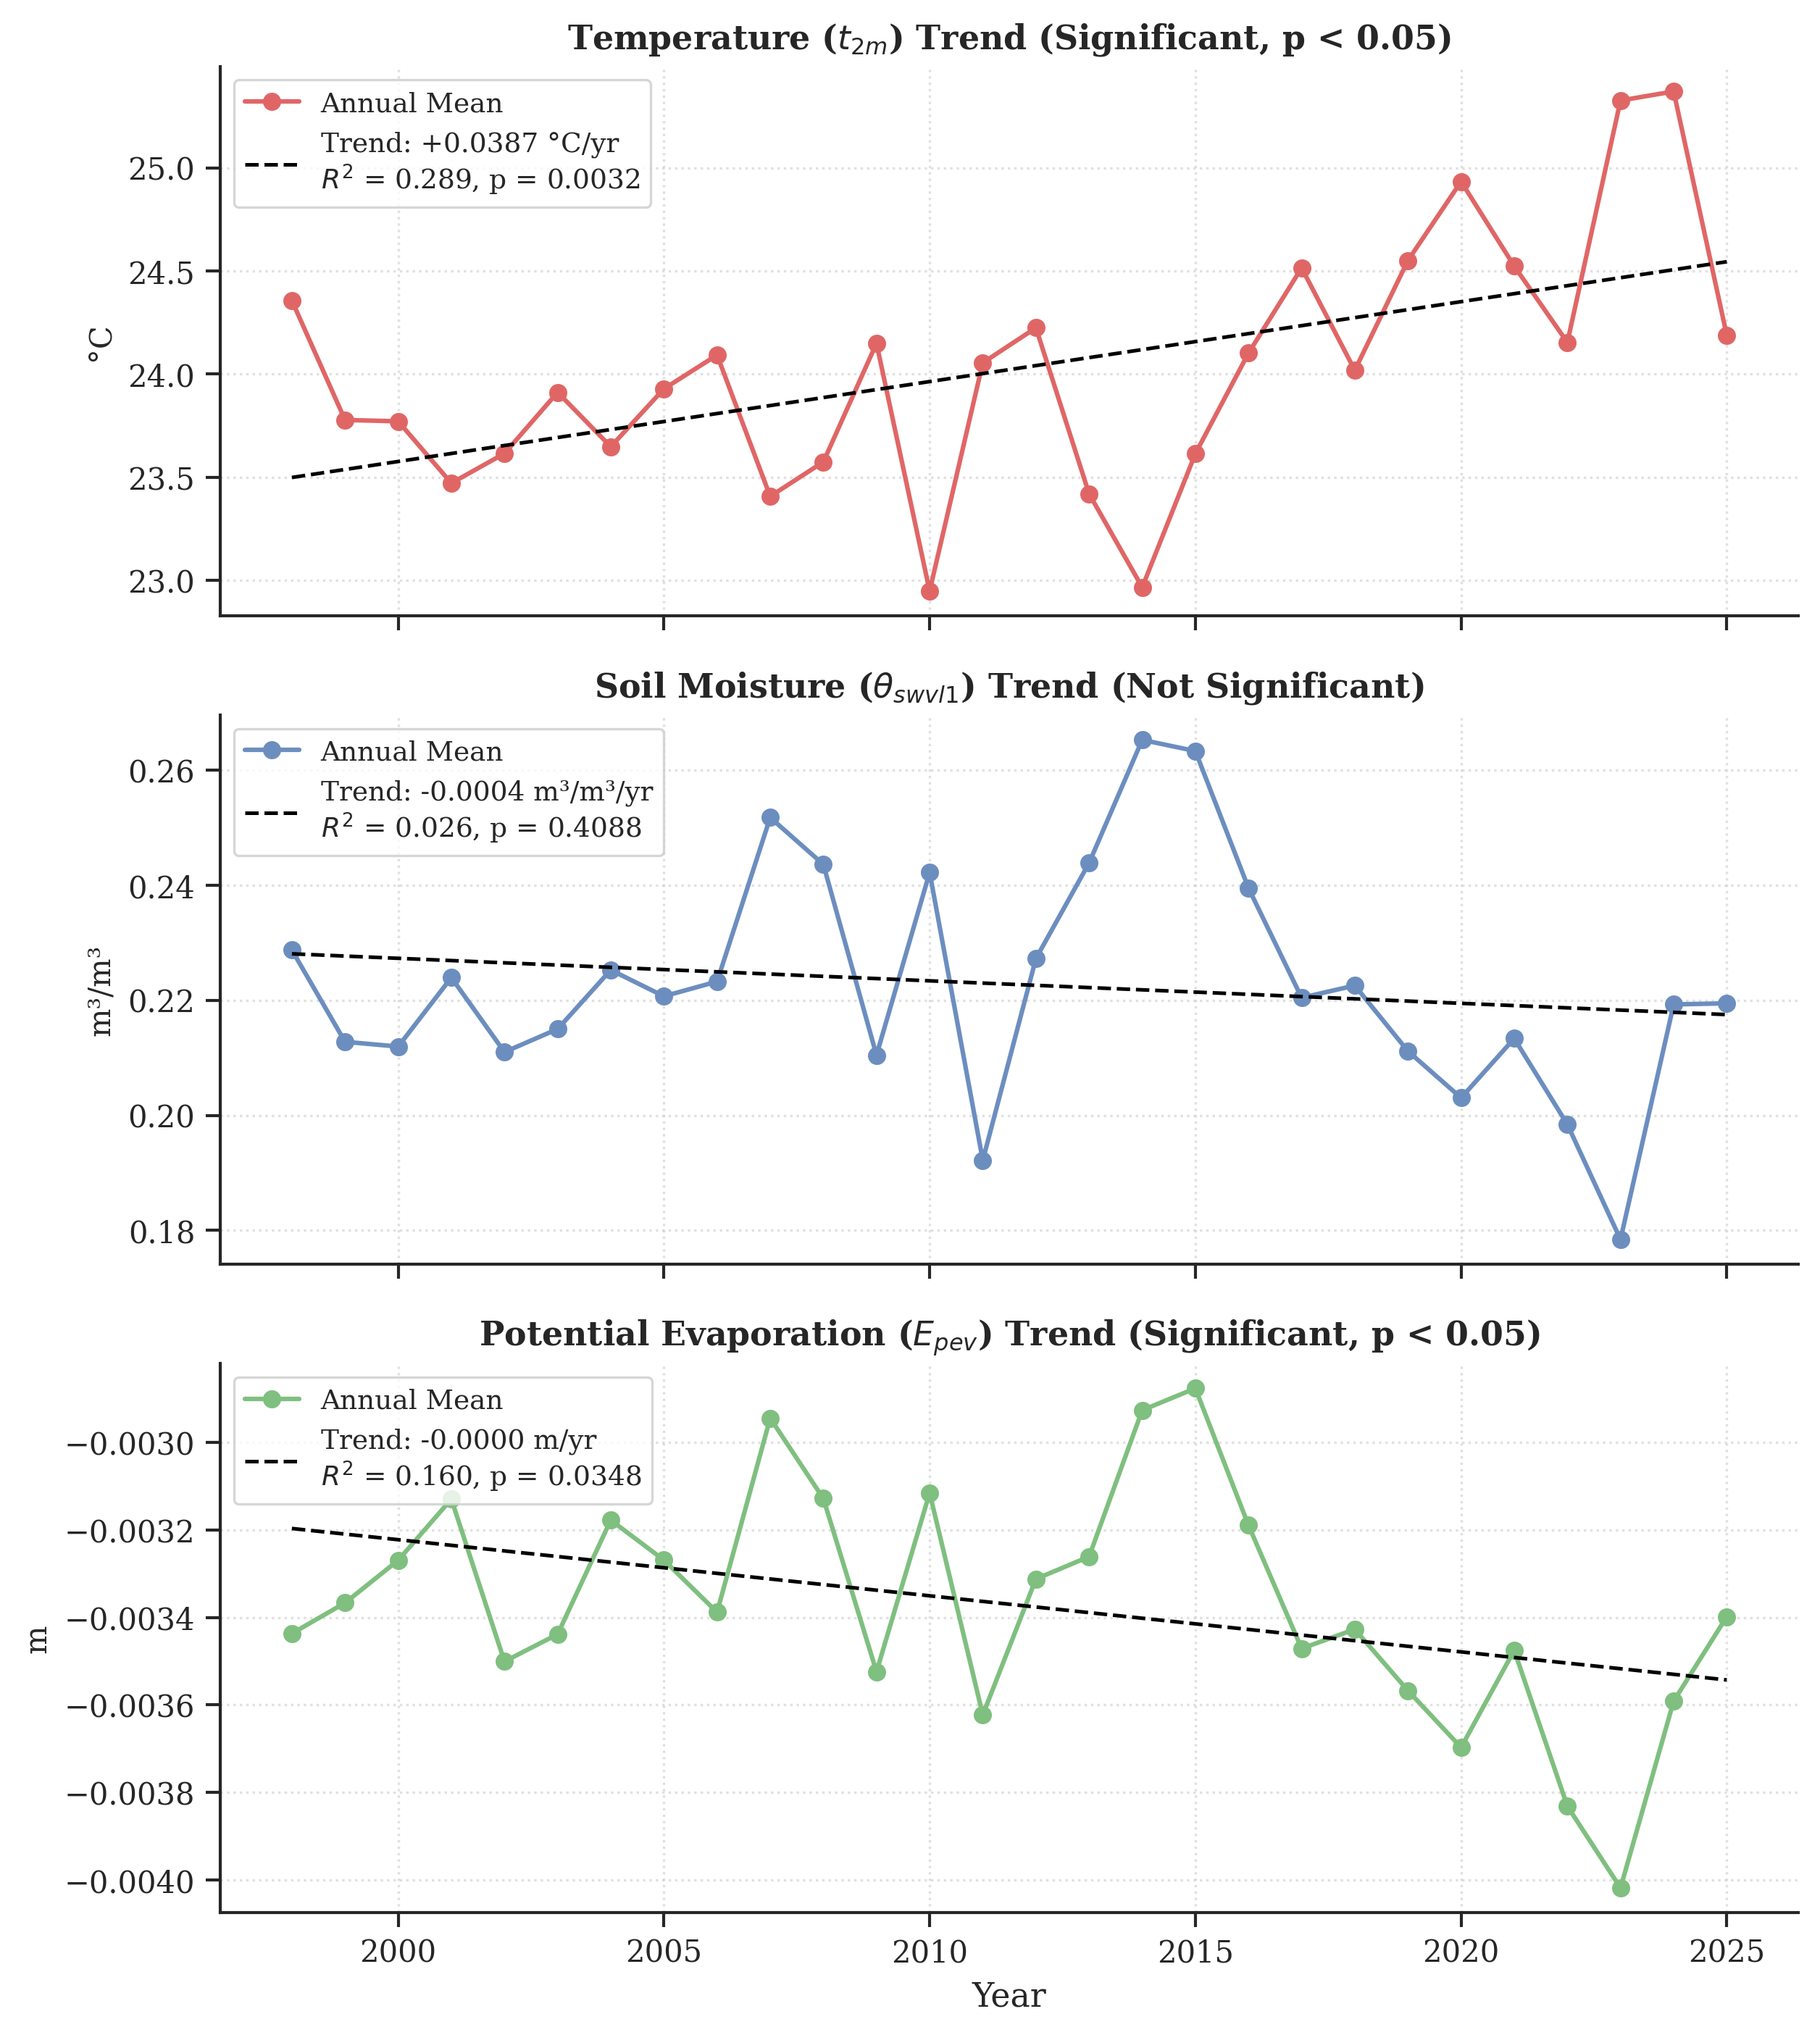
\includegraphics[width=\textwidth]{01_climatic_trends.png}
    \caption{Tendencias climáticas de largo plazo (1998--2025) para las tres variables de reanálisis ERA5-Land en la cuenca del Tamesí. Las líneas de regresión y los intervalos de confianza al 95\,\% se superponen a las medias anuales.}
    \label{fig:trends}
\end{figure}

\subsection{Estructura multivariante y análisis de componentes principales}
\label{subsec:pca}

El Análisis de Componentes Principales (ACP) sobre las variables escaladas indica que los dos primeros componentes explican el 86.7\,\% de la varianza total en el espacio tridimensional (Tabla~\ref{tab:pca} y Figura~\ref{fig:correlation}).

\begin{table}[H]
\centering
\caption{Cargas de los componentes principales y varianza explicada}
\label{tab:pca}
\small
\begin{tabular}{@{}lccccc@{}}
\toprule
Componente & Varianza (\%) & Carga $t2m$ & Carga $swvl1$ & Carga $pev$ & Interpretación \\
\midrule
PC1 & 52.87 & $-0.3677$ & $+0.5988$ & $+0.7115$ & Estado hídrico-evaporativo acoplado \\
PC2 & 33.83 & $+0.8456$ & $+0.5336$ & $-0.0121$ & Forzamiento térmico-hídrico \\
PC3 & 13.29 & $+0.3869$ & $-0.5972$ & $+0.7026$ & Residuos de demanda atmosférica \\
\bottomrule
\end{tabular}
\end{table}

PC1 representa el comportamiento hídrico-evaporativo acoplado del sistema suelo-vegetación-atmósfera. Las cargas positivas tanto para la humedad edáfica ($swvl1$) como para la evaporación potencial ($pev$, que en ERA5-Land se almacena con signo negativo, de modo que valores menos negativos indican menor demanda) señalan que las condiciones de suelo húmedo se acoplan con menor demanda evaporativa. PC2 está dominado por la temperatura ($+0.85$) y representa el componente independiente de forzamiento térmico.

Adicionalmente, los mapas de calor de correlación estacional (Figura~\ref{fig:correlation}) revelan patrones dinámicos clave en el acoplamiento suelo-atmósfera a lo largo del año. La correlación entre la temperatura ($t2m$) y la evaporación potencial ($pev$) es consistentemente fuerte y positiva (considerando la magnitud absoluta $|pev|$), lo que refleja que el forzamiento térmico es el principal motor de la demanda evaporativa atmosférica, alcanzando sus valores de Pearson más elevados durante la primavera (MAM, $r > 0.85$) y el verano (JJA, $r > 0.90$). Por otro lado, la relación entre la humedad edáfica superficial ($swvl1$) y la temperatura presenta una marcada variabilidad estacional. Durante la transición seca de primavera (MAM), se observa una correlación negativa moderada a fuerte, lo que evidencia el acoplamiento bidireccional donde la depleción de agua en el suelo limita el enfriamiento por evaporación latente, transfiriendo la energía disponible hacia el flujo de calor sensible y elevando la temperatura del aire. En contraste, durante el invierno (DEF), esta correlación se debilita notablemente debido a que la dinámica térmica es dominada por sistemas sinópticos externos (frentes fríos o ``nortes'') y no por retroalimentaciones locales de la superficie. Finalmente, la correlación negativa entre la humedad del suelo y la demanda evaporativa absoluta se intensifica en el verano y otoño (SON), periodos donde los eventos de precipitación intensa saturan el perfil del suelo y, simultáneamente, incrementan la cobertura nubosa y la humedad relativa, atenuando la demanda atmosférica.

\begin{figure}[H]
    \centering
    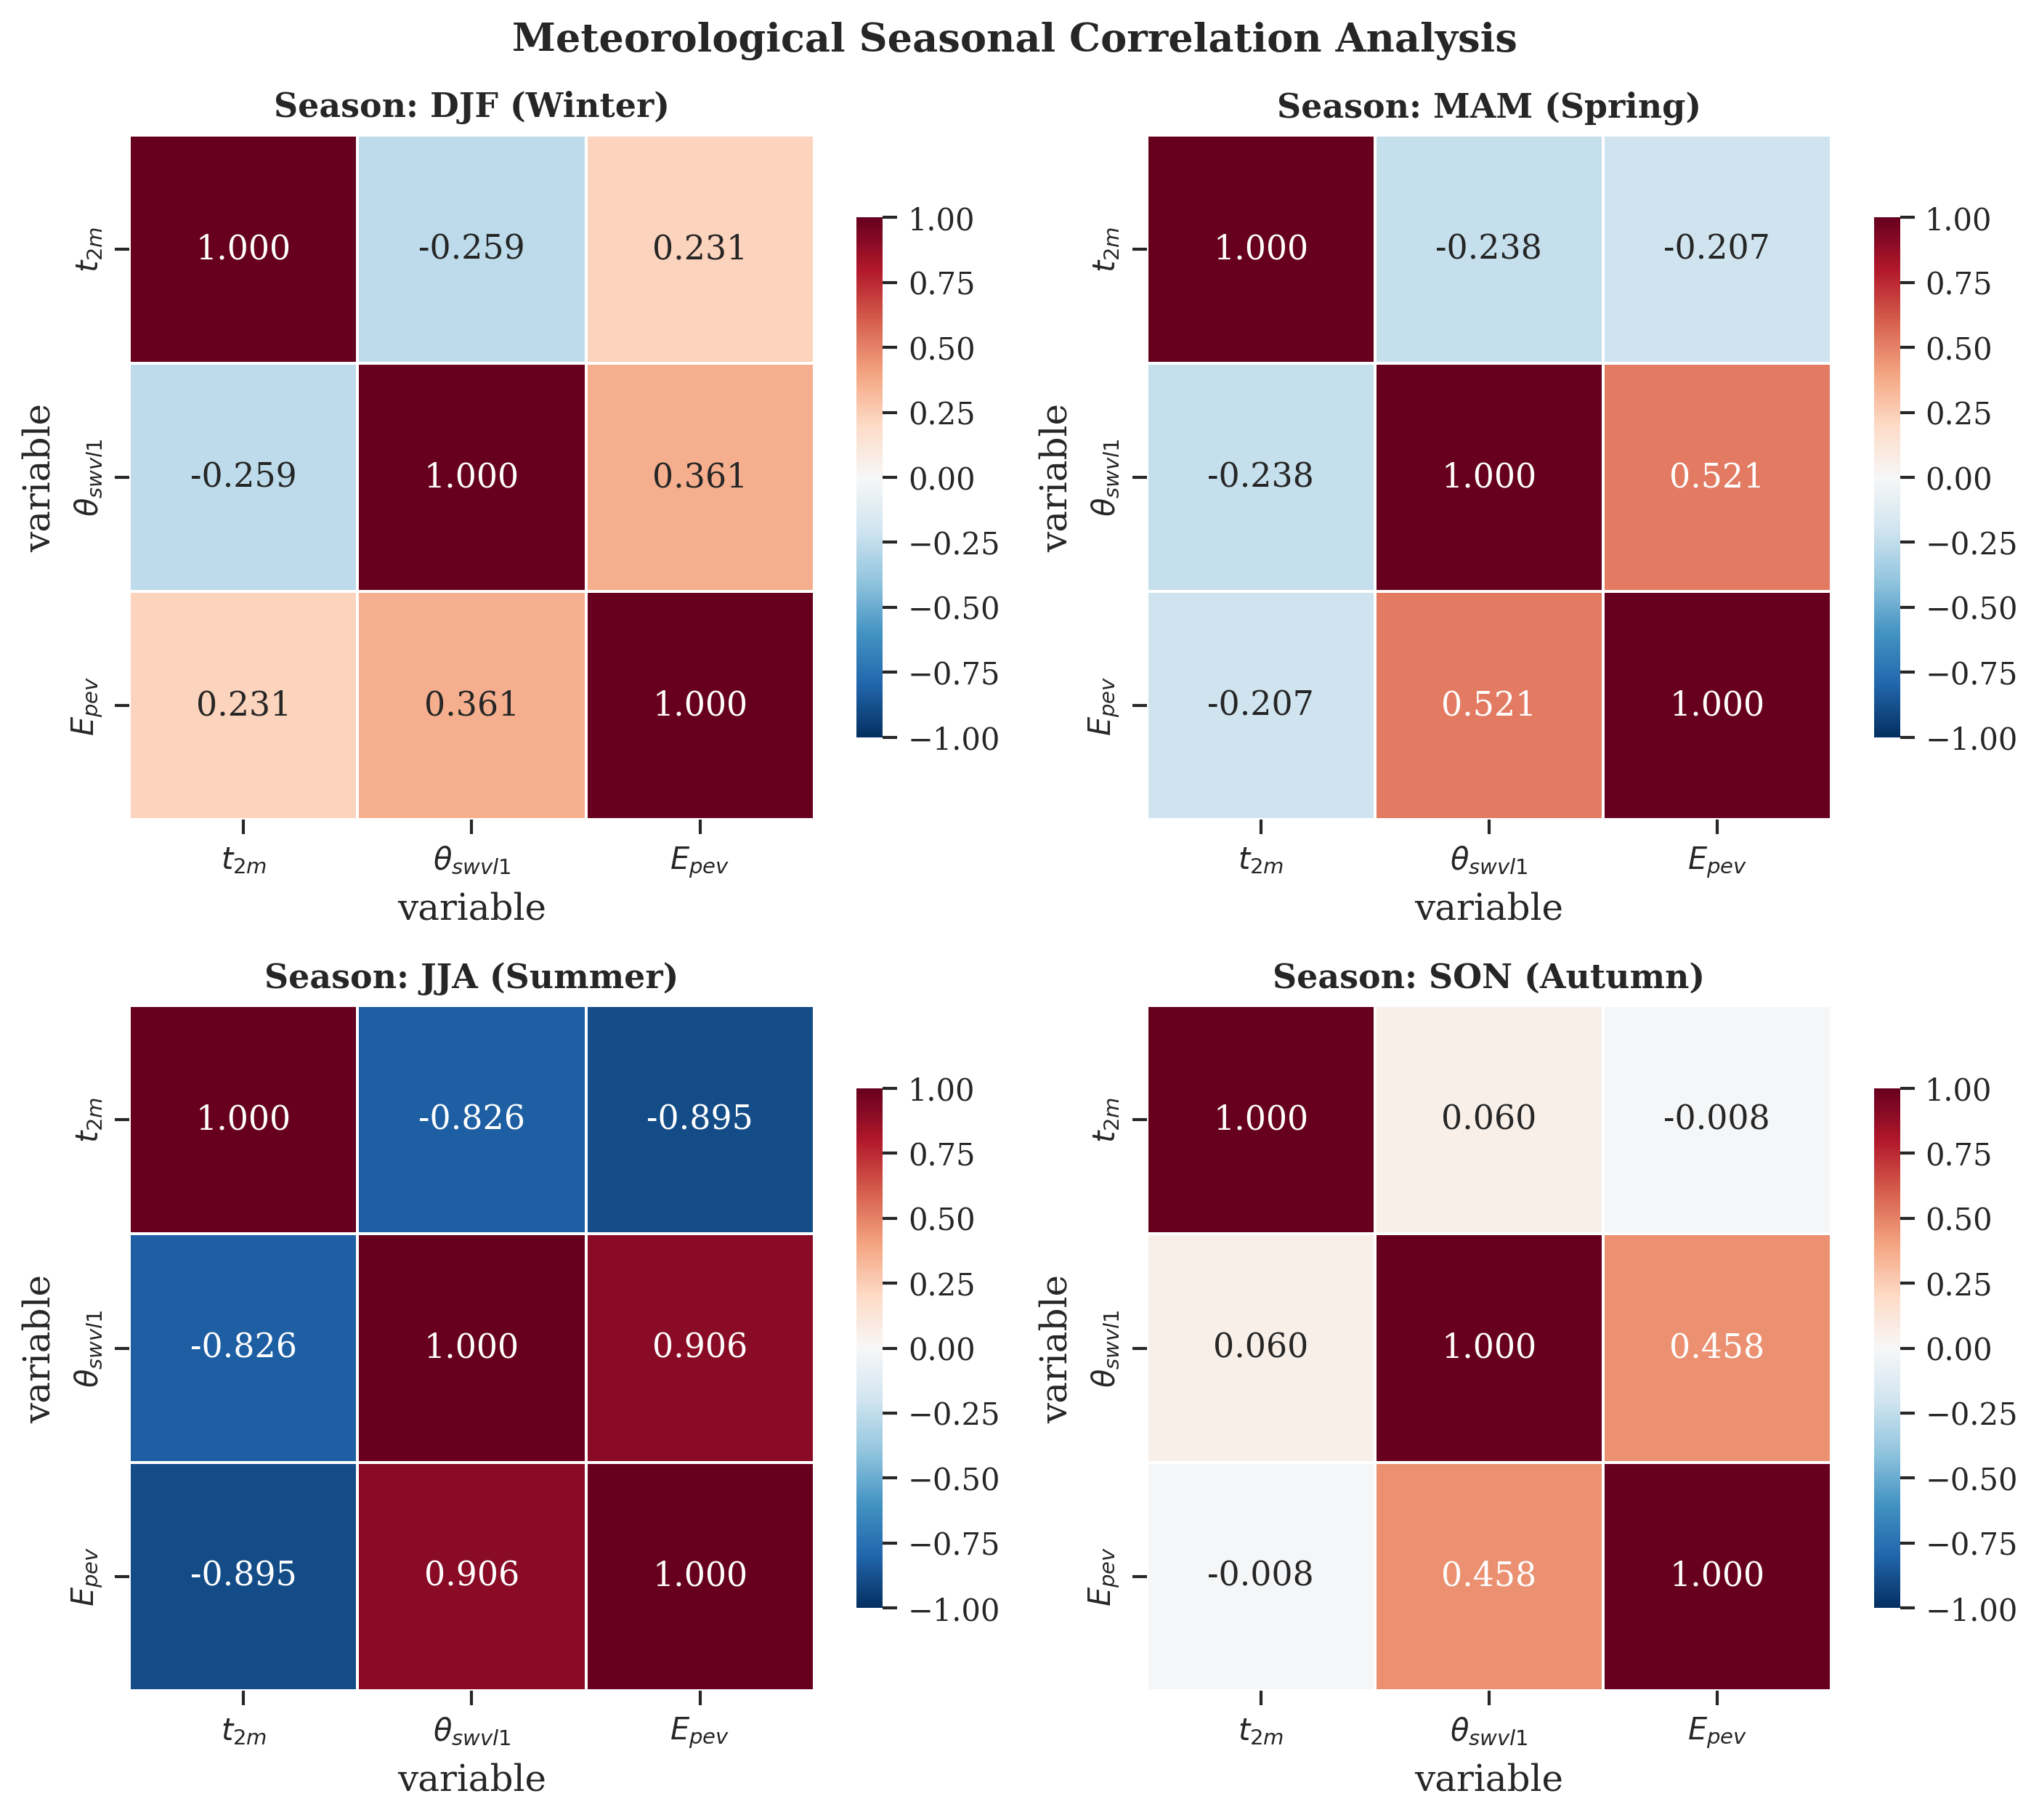
\includegraphics[width=\textwidth]{02_seasonal_correlation.png}
    \caption{Mapas de calor de correlación estacional entre las tres variables de reanálisis. Las correlaciones de Pearson se calcularon de forma independiente para cada estación meteorológica (DEF, MAM, JJA, SON).}
    \label{fig:correlation}
\end{figure}

\subsection{Desempeño de los modelos de aprendizaje automático}
\label{subsec:ml_results}

Ambos modelos exhibieron un desempeño elevado en todos los pliegues de validación cruzada, lo que demuestra que las variables predictoras derivadas contienen señales predictivas robustas. El GBR superó consistentemente al RF en todos los pliegues (Tabla~\ref{tab:cv}).

\begin{table}[H]
\centering
\caption{Comparación de validación cruzada temporal: RF frente a GBR}
\label{tab:cv}
\small
\begin{tabular}{@{}clcccc@{}}
\toprule
Pliegue & Periodo de prueba & RMSE (RF) & RMSE (GBR) & $R^2$ (RF) & $R^2$ (GBR) \\
\midrule
1 & 2002-09 $\to$ 2007-05 & 0.0150 & 0.0105 & 0.9817 & 0.9911 \\
2 & 2007-05 $\to$ 2011-12 & 0.0138 & 0.0085 & 0.9876 & 0.9952 \\
3 & 2011-12 $\to$ 2016-08 & 0.0107 & 0.0066 & 0.9916 & 0.9968 \\
4 & 2016-08 $\to$ 2021-03 & 0.0089 & 0.0051 & 0.9937 & 0.9979 \\
5 & 2021-03 $\to$ 2025-12 & 0.0095 & 0.0053 & 0.9937 & 0.9981 \\
\midrule
\textbf{Media} & --- & \textbf{0.0116} & \textbf{0.0072} & \textbf{0.9897} & \textbf{0.9958} \\
\bottomrule
\end{tabular}
\end{table}

El GBR redujo el RMSE medio en un 37.9\,\% respecto al RF (de 0.0116 a 0.0072) y alcanzó un $R^2$ medio de 0.9958. Este resultado indica que el mecanismo de aprendizaje secuencial de residuos del \emph{boosting} resulta altamente efectivo para capturar las no linealidades a escala fina en la retroalimentación suelo-atmósfera.

\begin{figure}[H]
    \centering
    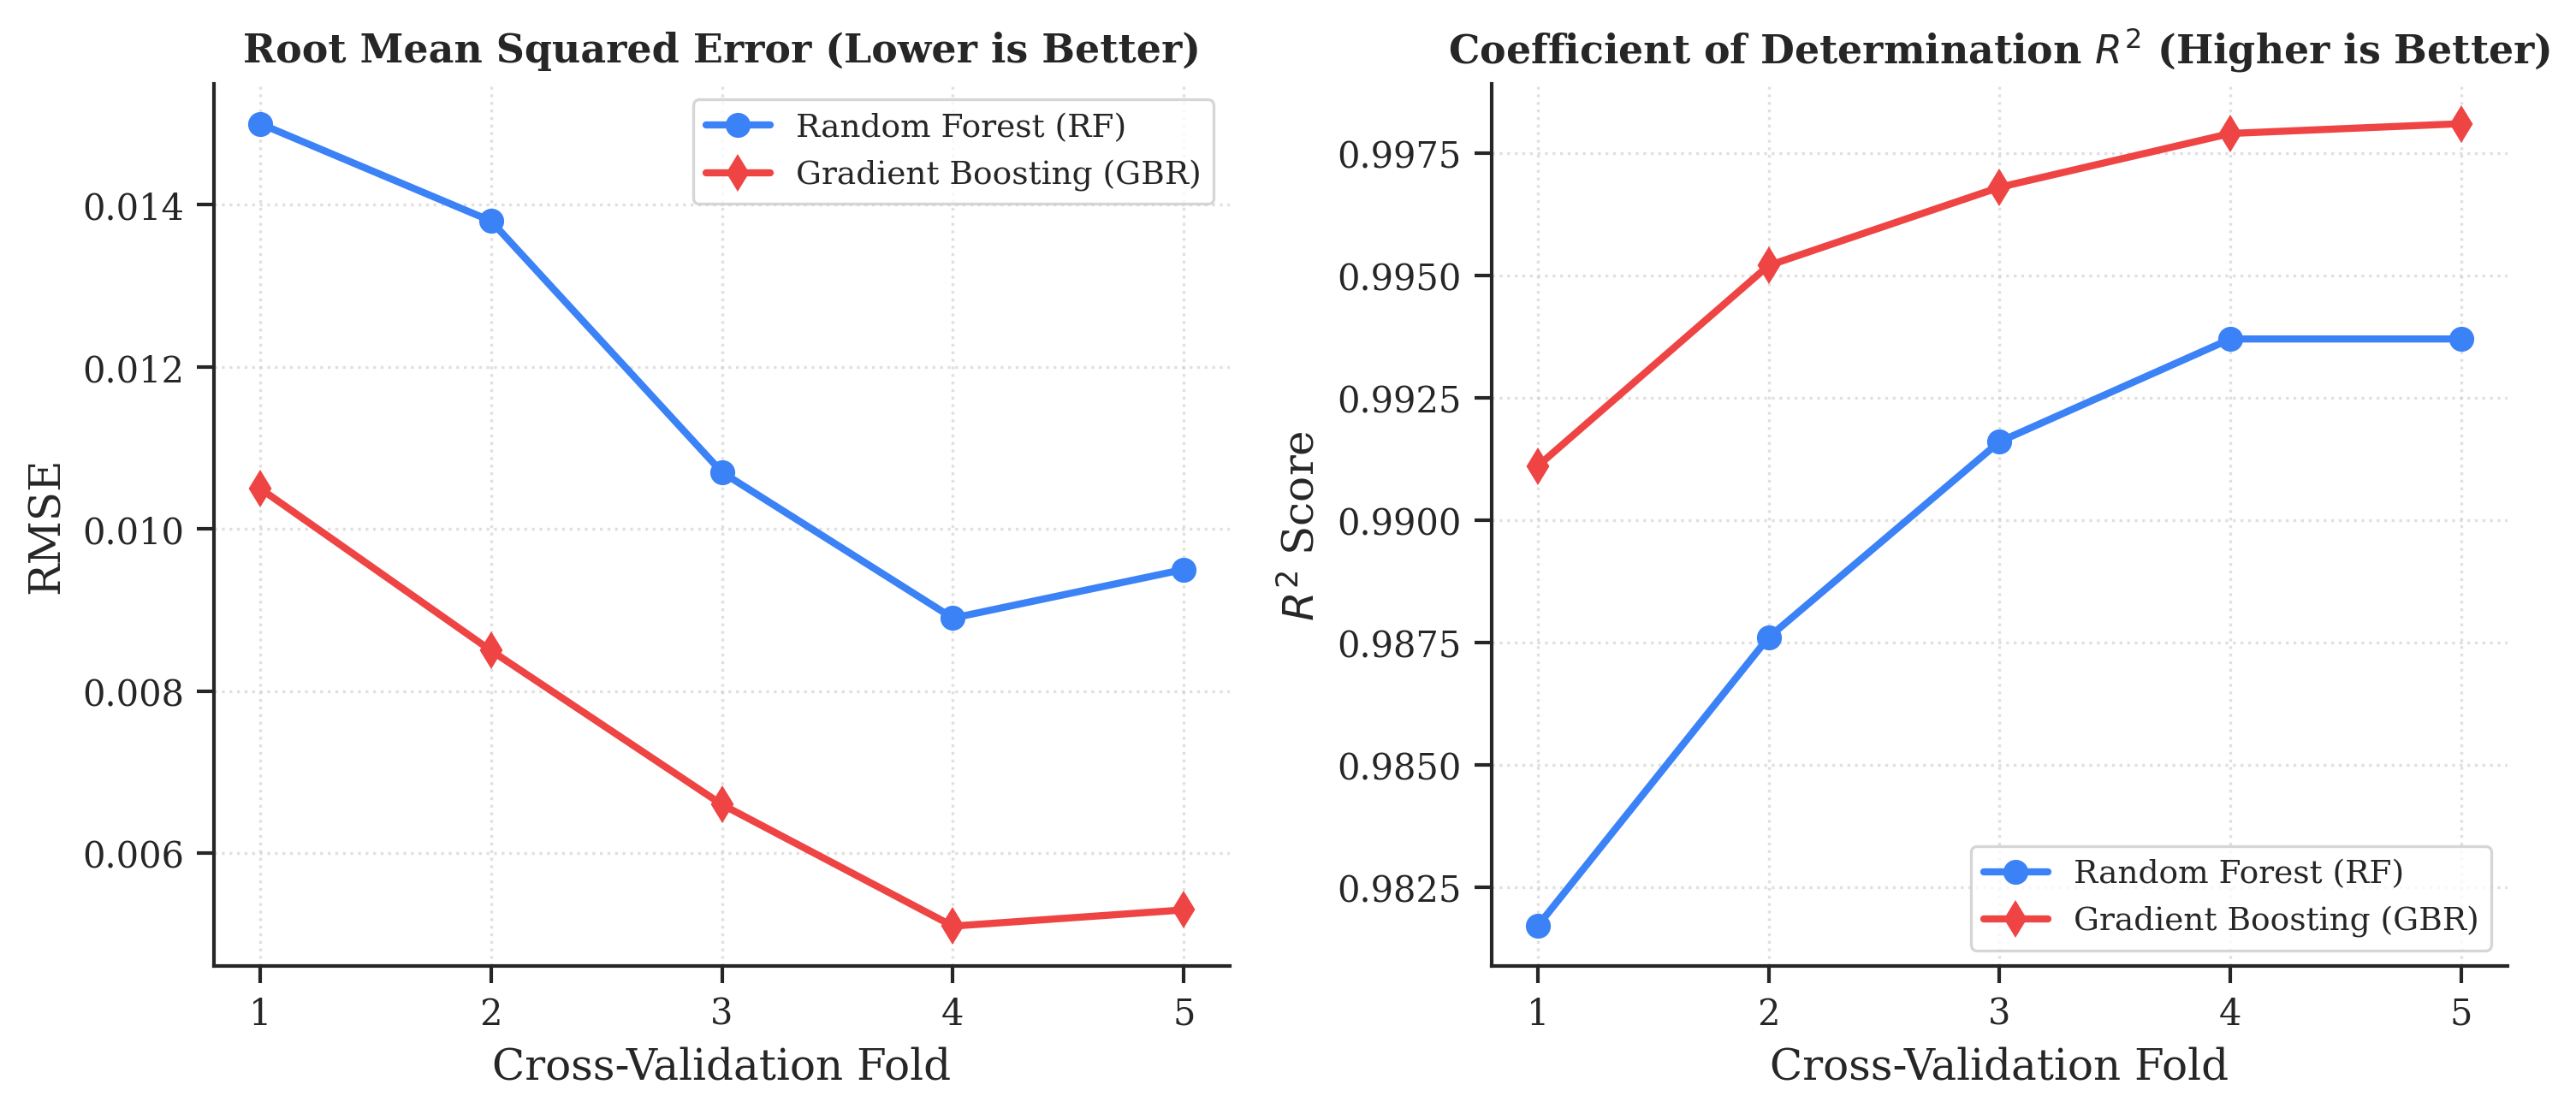
\includegraphics[width=\textwidth]{04_ml_comparison.png}
    \caption{Métricas de validación cruzada temporal por pliegue para los modelos RF y GBR.}
    \label{fig:ml_comparison}
\end{figure}

El análisis de importancia de variables mediante Gini y SHAP demostró que el índice térmico-hídrico ($T_{2m}/\theta_{\text{swvl1}}$) y las anomalías de evaporación potencial constituyen las variables más determinantes para explicar la varianza del índice. Este hallazgo confirma que la captura de acoplamientos físicos mediante cocientes resulta superior a la alimentación directa de variables crudas al modelo.

\begin{figure}[H]
    \centering
    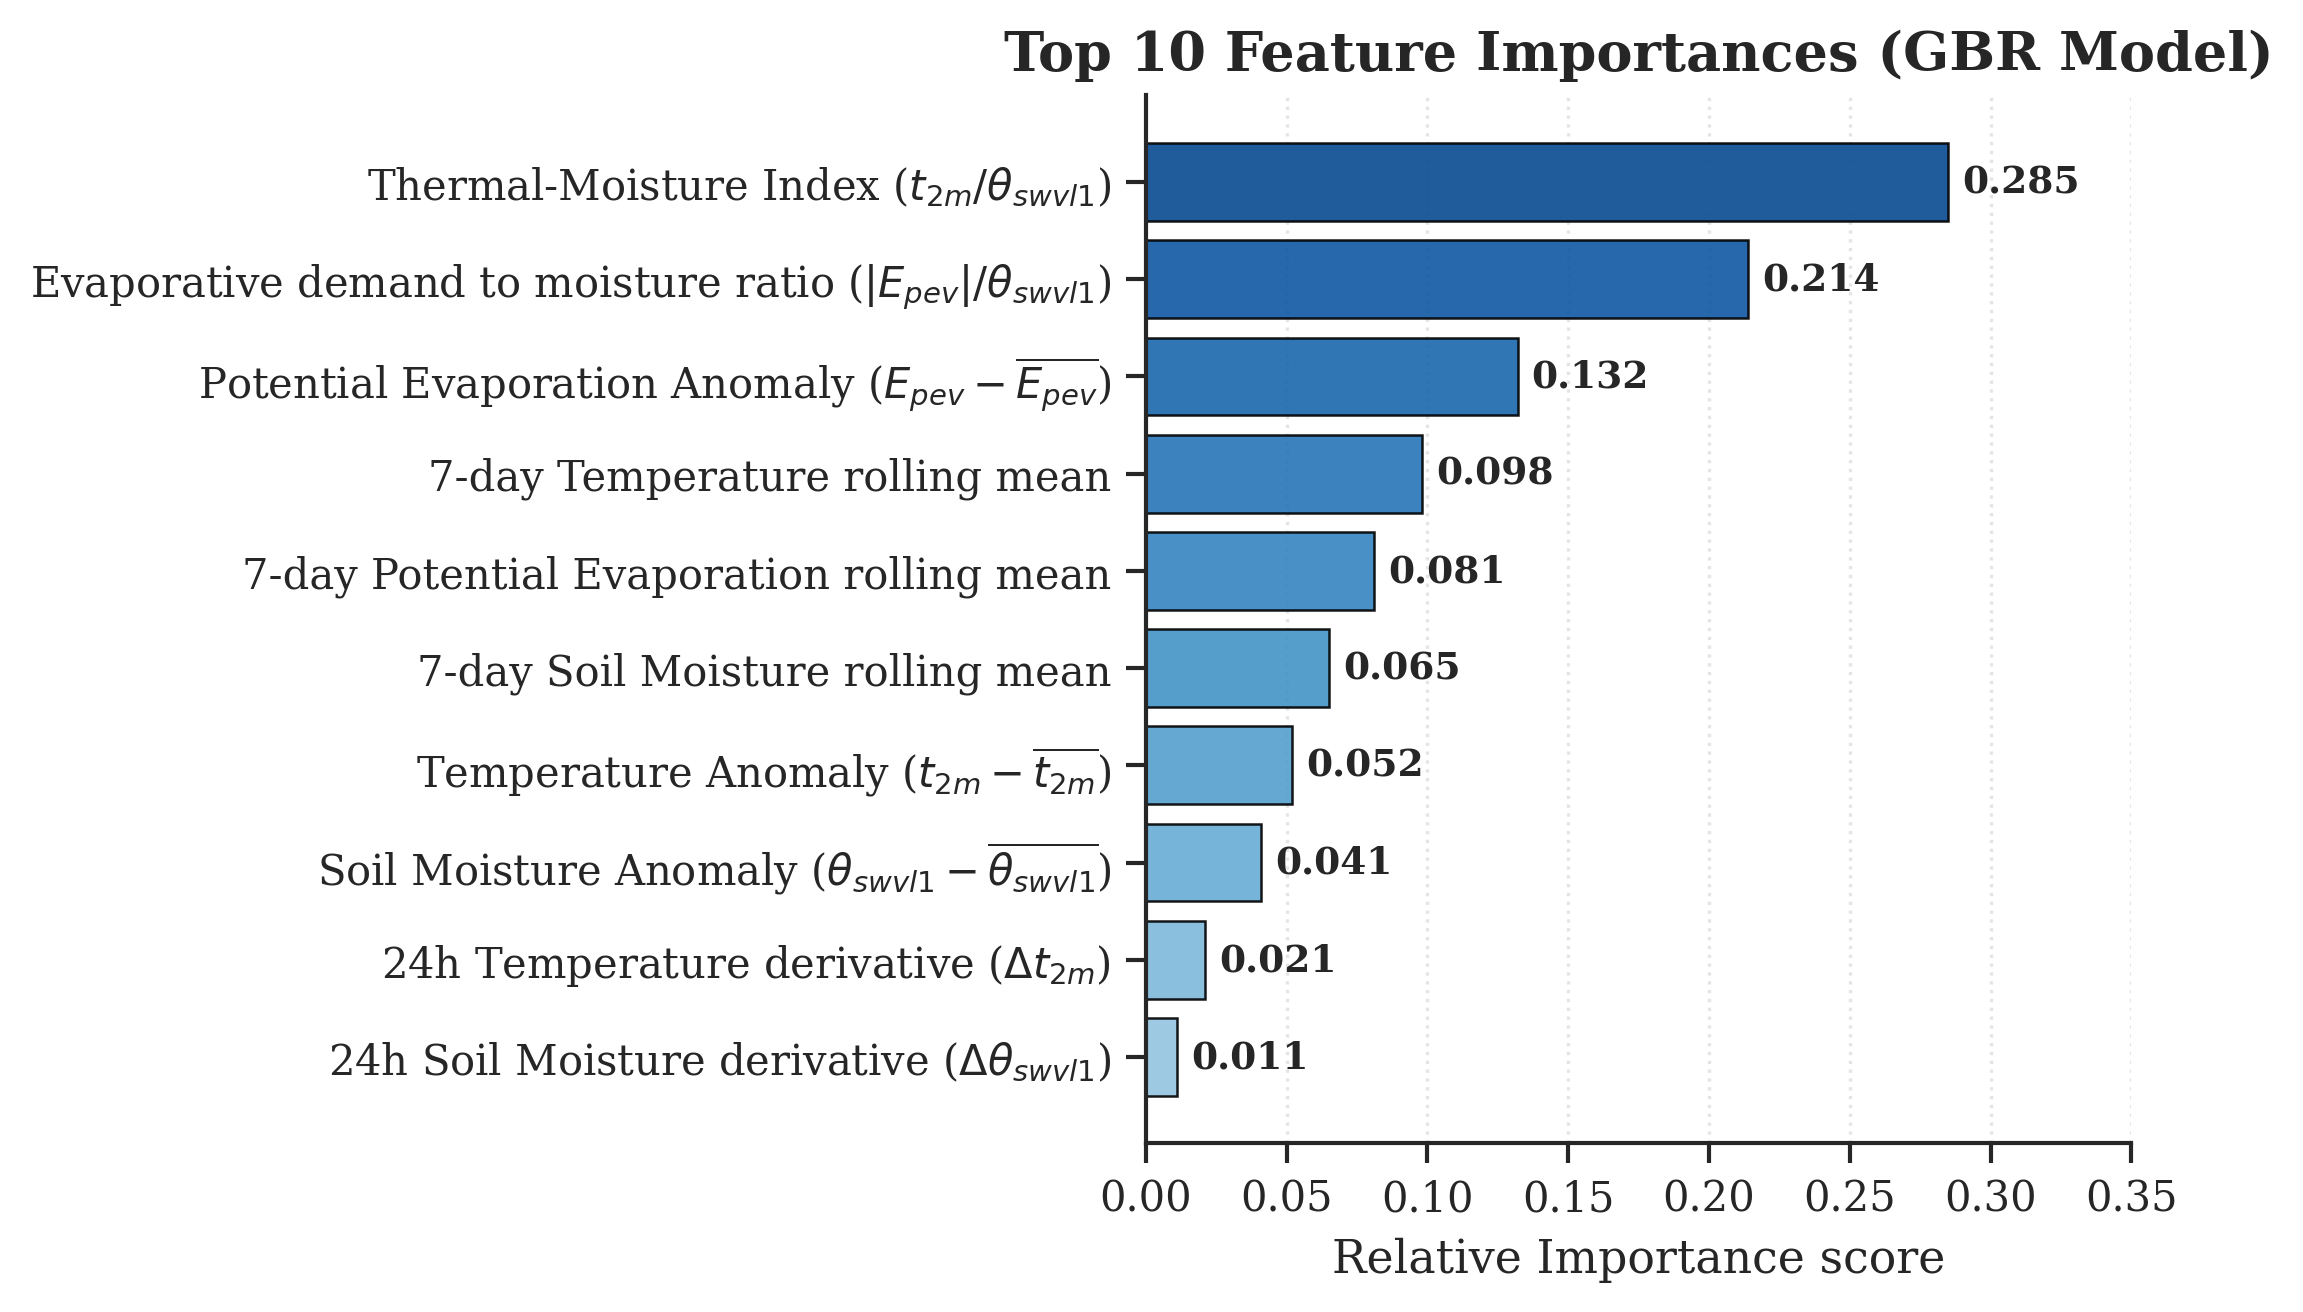
\includegraphics[width=0.85\textwidth]{05_feature_importances.png}
    \caption{Importancia de las 10 principales variables predictoras del modelo GBR, calculada mediante la ganancia media de Gini.}
    \label{fig:importances}
\end{figure}

\subsection{Validación basada en eventos}
\label{subsec:event_val}

La validación de la serie CHSI reconstruida frente al catálogo de eventos extremos documentados mostró una \textbf{concordancia direccional del 100\,\%} (9 de 9 eventos clasificados correctamente), según se detalla en la Tabla~\ref{tab:eventos} y la Figura~\ref{fig:events}.

\begin{table}[H]
\centering
\caption{Validación del CHSI frente a eventos extremos documentados en la cuenca del Tamesí}
\label{tab:eventos}
\small
\begin{tabular}{@{}llccccc@{}}
\toprule
Evento & Tipo & Periodo & CHSI medio & Línea base & $Z$ & Resultado \\
\midrule
Sequía 1998--2003       & Sequía      & 1998-01 a 2003-12 & 0.5271 & 0.5173 & $+0.099$ & Correcto \\
Sequía excepcional 2011 & Sequía      & 2011-01 a 2012-06 & 0.5527 & 0.5173 & $+0.320$ & Correcto \\
Sequía severa 2022      & Sequía      & 2022-03 a 2022-09 & 0.6118 & 0.5173 & $+0.832$ & Correcto \\
Sequía excepcional 2024 & Sequía      & 2024-03 a 2024-09 & 0.5727 & 0.5173 & $+0.494$ & Correcto \\
Huracán Keith 2000      & Inundación  & 2000-10-01 a 10-15 & 0.4011 & 0.5173 & $-0.993$ & Correcto \\
Inundaciones jul. 2007  & Inundación  & 2007-07            & 0.4995 & 0.5173 & $-0.141$ & Correcto \\
Huracán Alex 2010       & Inundación  & 2010-06-15 a 07-15 & 0.4683 & 0.5173 & $-0.412$ & Correcto \\
Huracán Ingrid 2013     & Inundación  & 2013-09-15 a 10-15 & 0.3913 & 0.5173 & $-1.079$ & Correcto \\
Inundaciones 2017       & Inundación  & 2017-09-20 a 10-10 & 0.4292 & 0.5173 & $-0.750$ & Correcto \\
\bottomrule
\end{tabular}
\end{table}

\begin{figure}[H]
    \centering
    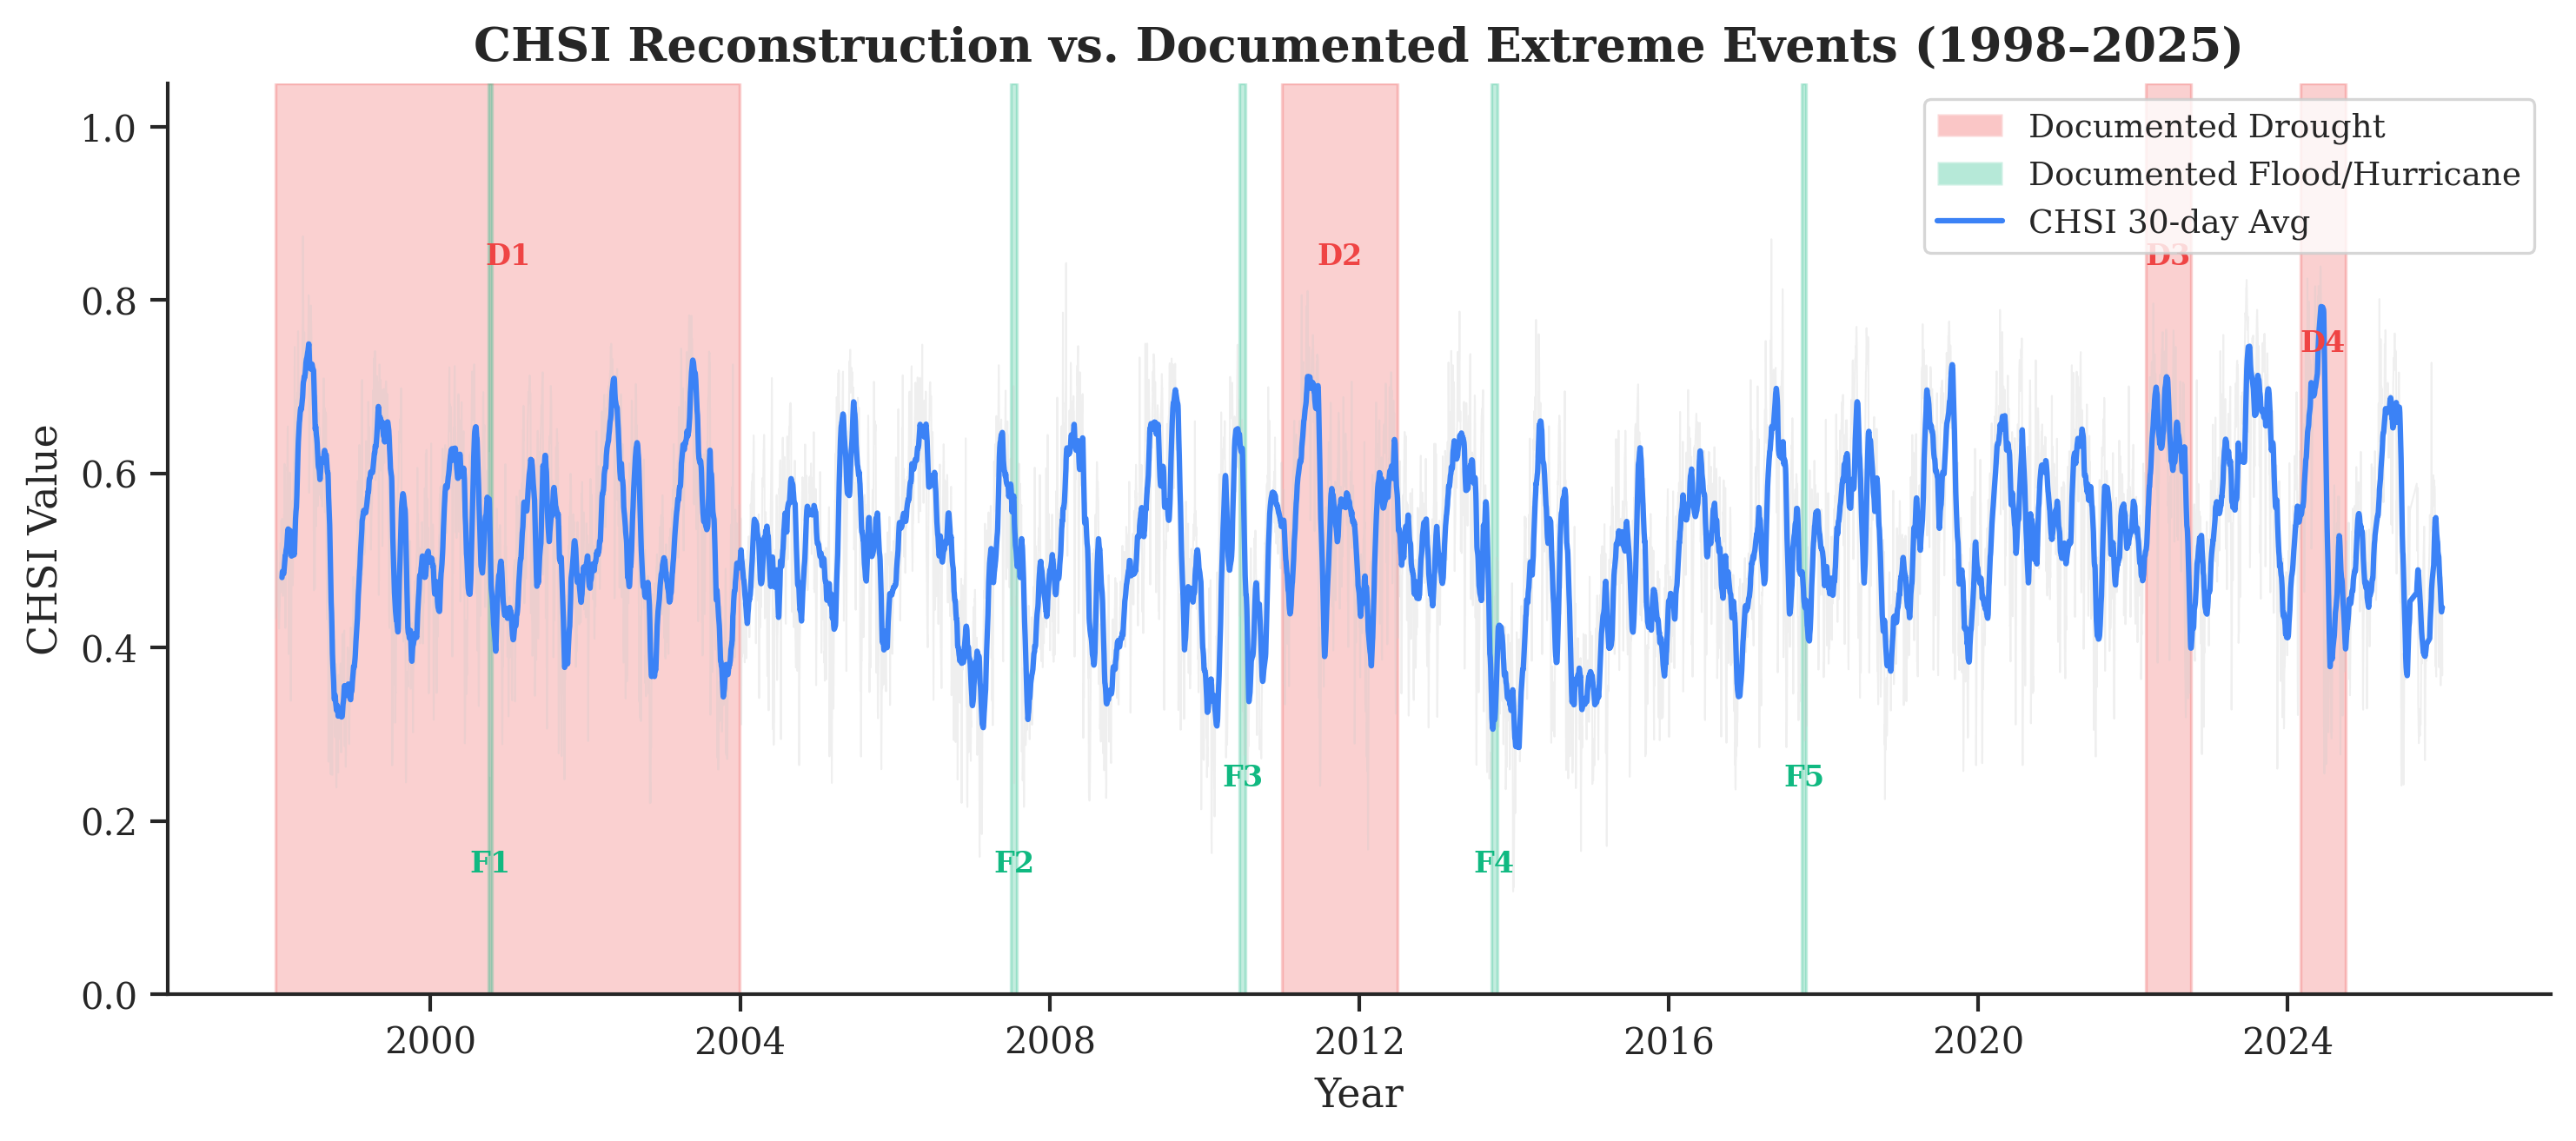
\includegraphics[width=\textwidth]{03_chsi_events.png}
    \caption{Serie temporal del CHSI reconstruido (1998--2025) con anotaciones de los nueve eventos extremos documentados. Las bandas sombreadas indican periodos de sequía (rojo) e inundación (azul).}
    \label{fig:events}
\end{figure}

\subsection{Análisis de tendencias por ventana móvil y velocidad de estrés hídrico}
\label{subsec:mwt}

Para comprender la trayectoria temporal y la tasa de cambio del CHSI, se realizó un análisis de tendencias por ventana móvil (\emph{Moving-Window Trend}, MWT) con dos ventanas centradas:

\begin{enumerate}
    \item \textbf{Ventana estacional (90~días):} Captura la tasa de cambio sub-estacional, definida como la \emph{velocidad de acumulación de estrés hídrico}.
    \item \textbf{Ventana anual (365~días):} Captura la tasa de cambio interanual, definida como la \emph{velocidad de tendencia anual del estrés hídrico}, filtrando los ciclos estacionales.
\end{enumerate}

La tendencia lineal global del CHSI reconstruido es positiva y altamente significativa:
%
\begin{equation}
    \text{Pendiente}_{\text{global}} = +0.001100\;\text{año}^{-1} \quad (R^2 = 0.0056,\; p < 0.0001)
    \label{eq:trend_global}
\end{equation}
%
Este resultado indica un desplazamiento multidecadal sostenido hacia niveles superiores de estrés hídrico a lo largo de los 28~años (un incremento acumulado de aproximadamente $+0.0308$ en el índice).

A escala estacional (Figura~\ref{fig:seasonal_slopes}), las pendientes exhiben alta volatilidad, reflejando transiciones rápidas en la hidrología de la cuenca. Durante eventos de inundación, las pendientes negativas son dominadas por incrementos acelerados de humedad edáfica (pendientes de sequedad del suelo de hasta $-4.6958$~año$^{-1}$). Durante las fases de inicio de sequía, la acumulación de estrés se impulsa por un aumento concurrente de la sequedad edáfica y la evaporación potencial.

\begin{figure}[H]
    \centering
    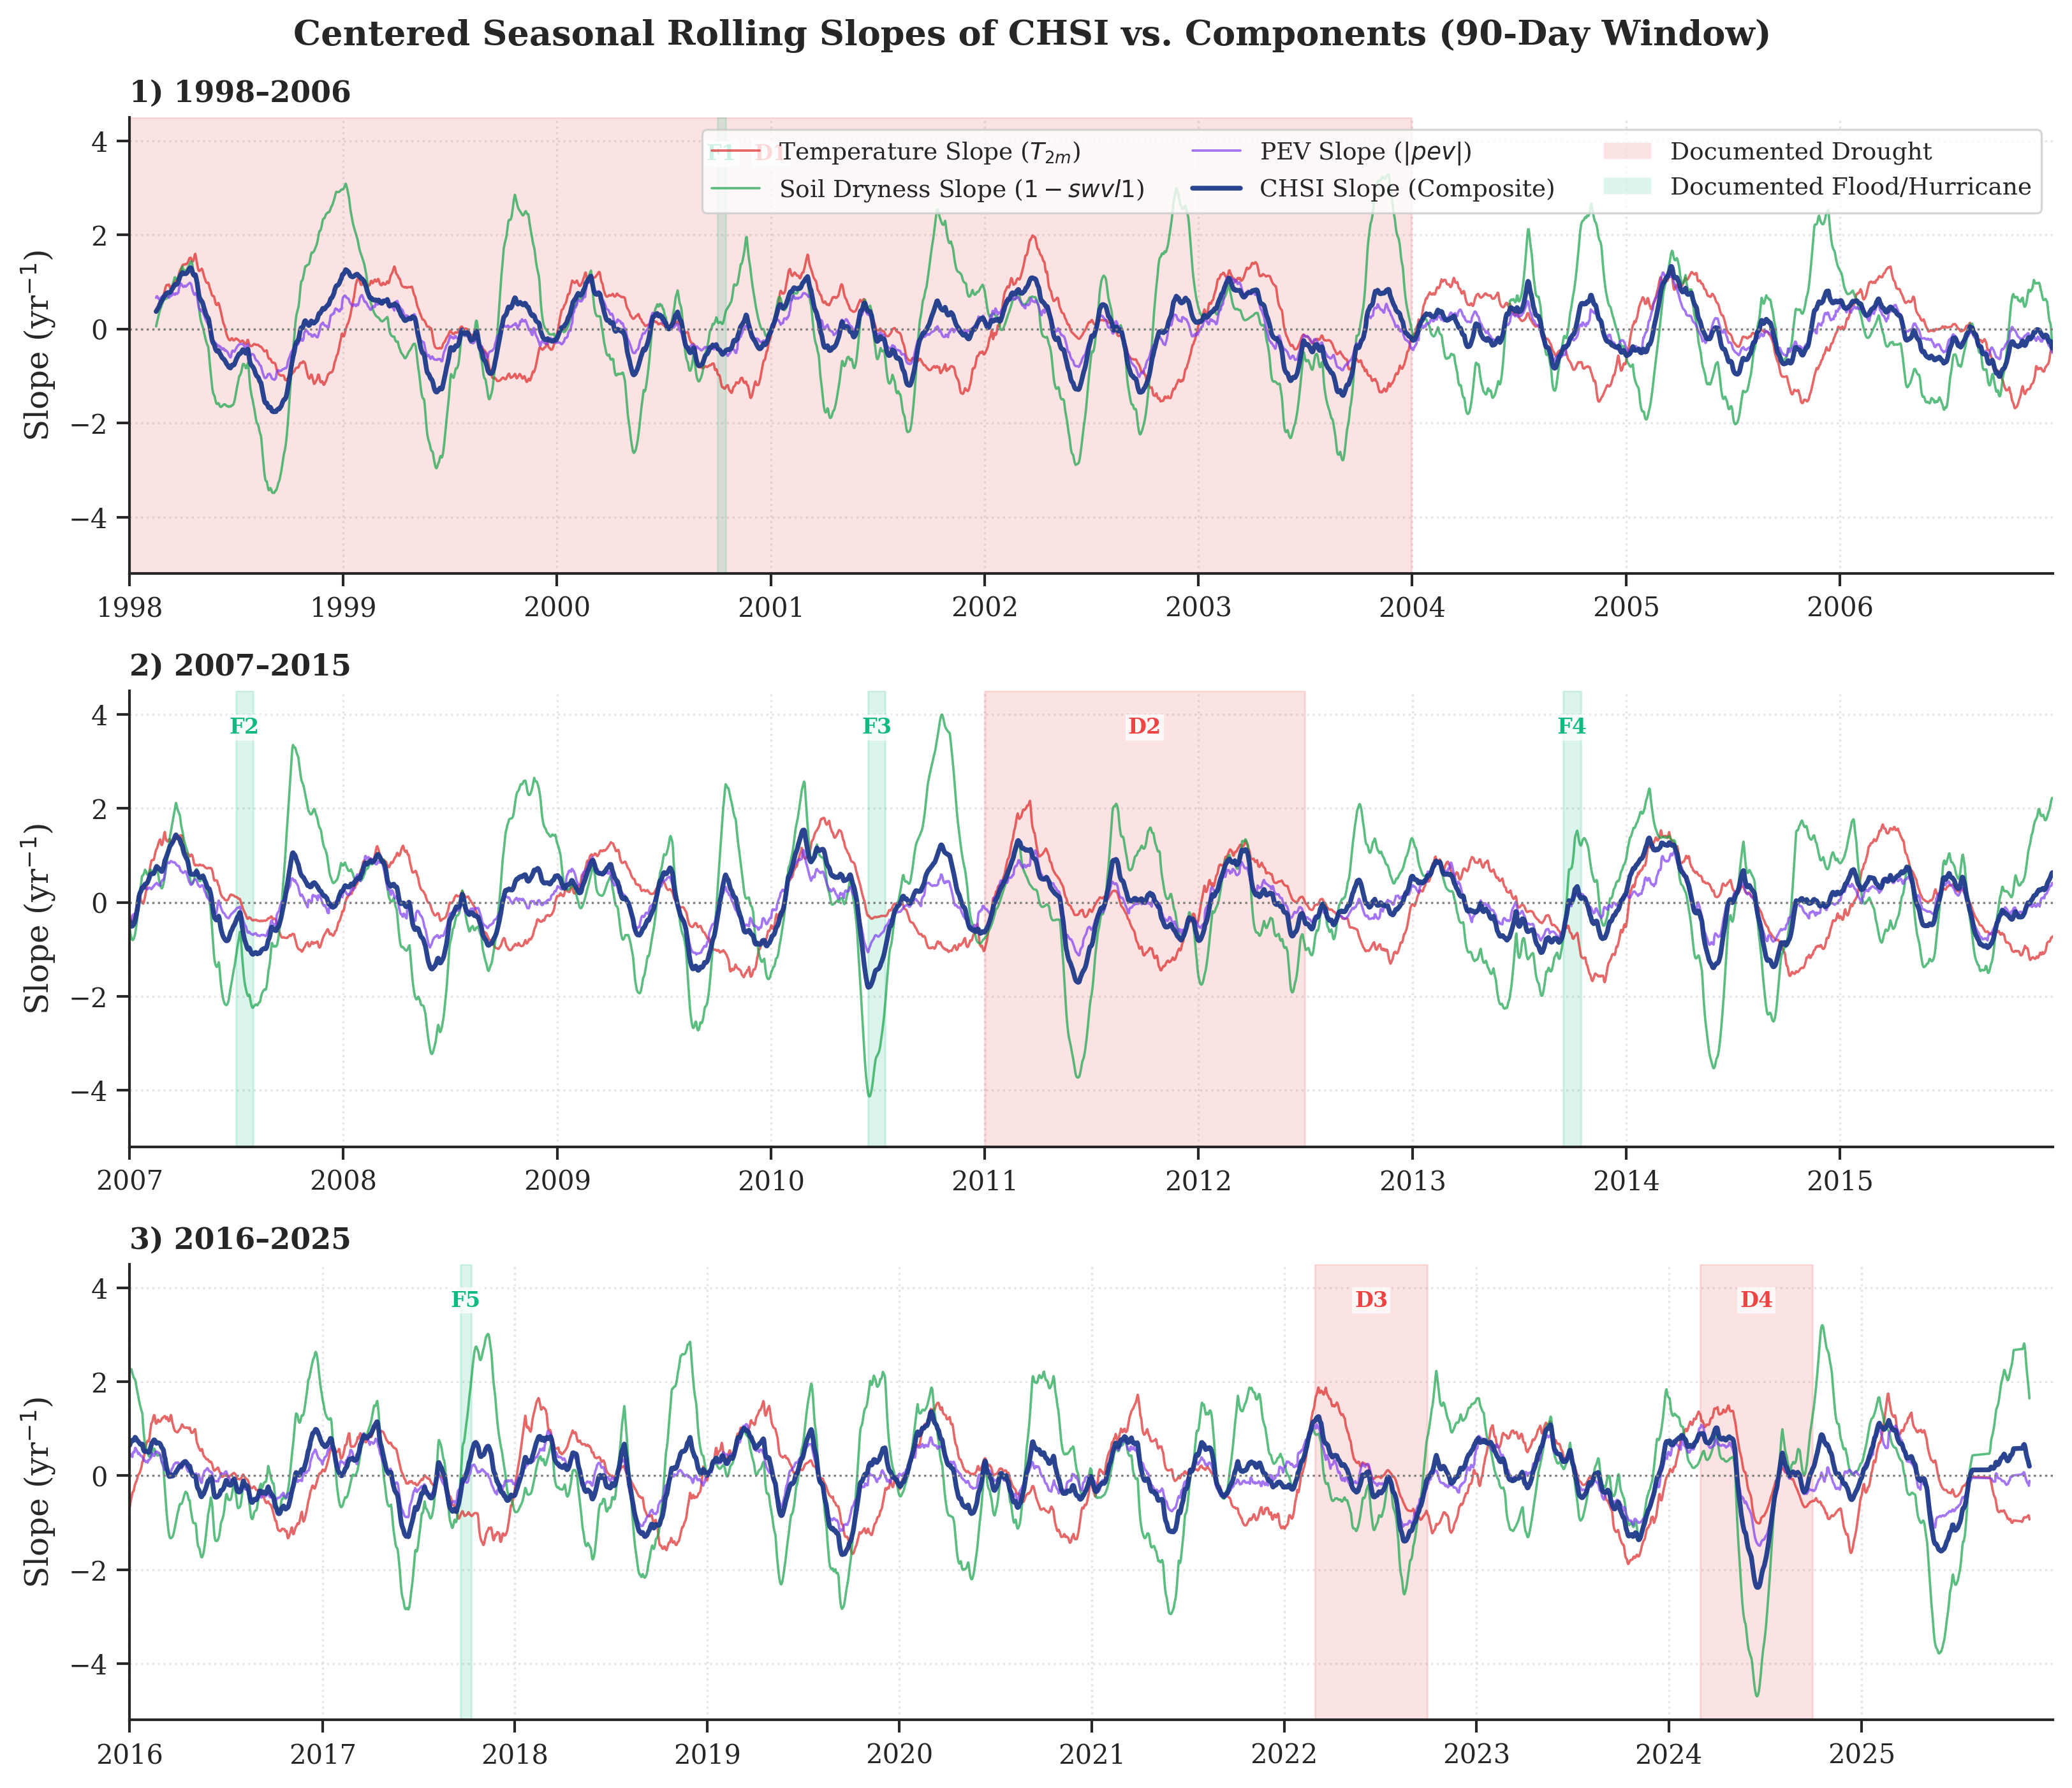
\includegraphics[width=\textwidth]{06_chsi_seasonal_slopes_comparison.png}
    \caption{Pendientes de regresión estacional centrada (ventana de 90~días) del CHSI y sus componentes normalizados, segmentadas en tres paneles cronológicos.}
    \label{fig:seasonal_slopes}
\end{figure}

A escala anual (Figura~\ref{fig:yearly_slopes}), el ruido estacional se filtra y se revela la tasa sostenida de acumulación de estrés interanual. La pendiente anual máxima del CHSI se registró el 24 de febrero de~2009 ($+0.35861$~año$^{-1}$), dominada por la depleción de humedad edáfica ($+0.54017$~año$^{-1}$), acompañada por calentamiento ($+0.27577$~año$^{-1}$) y demanda evaporativa ($+0.25990$~año$^{-1}$).

\begin{figure}[H]
    \centering
    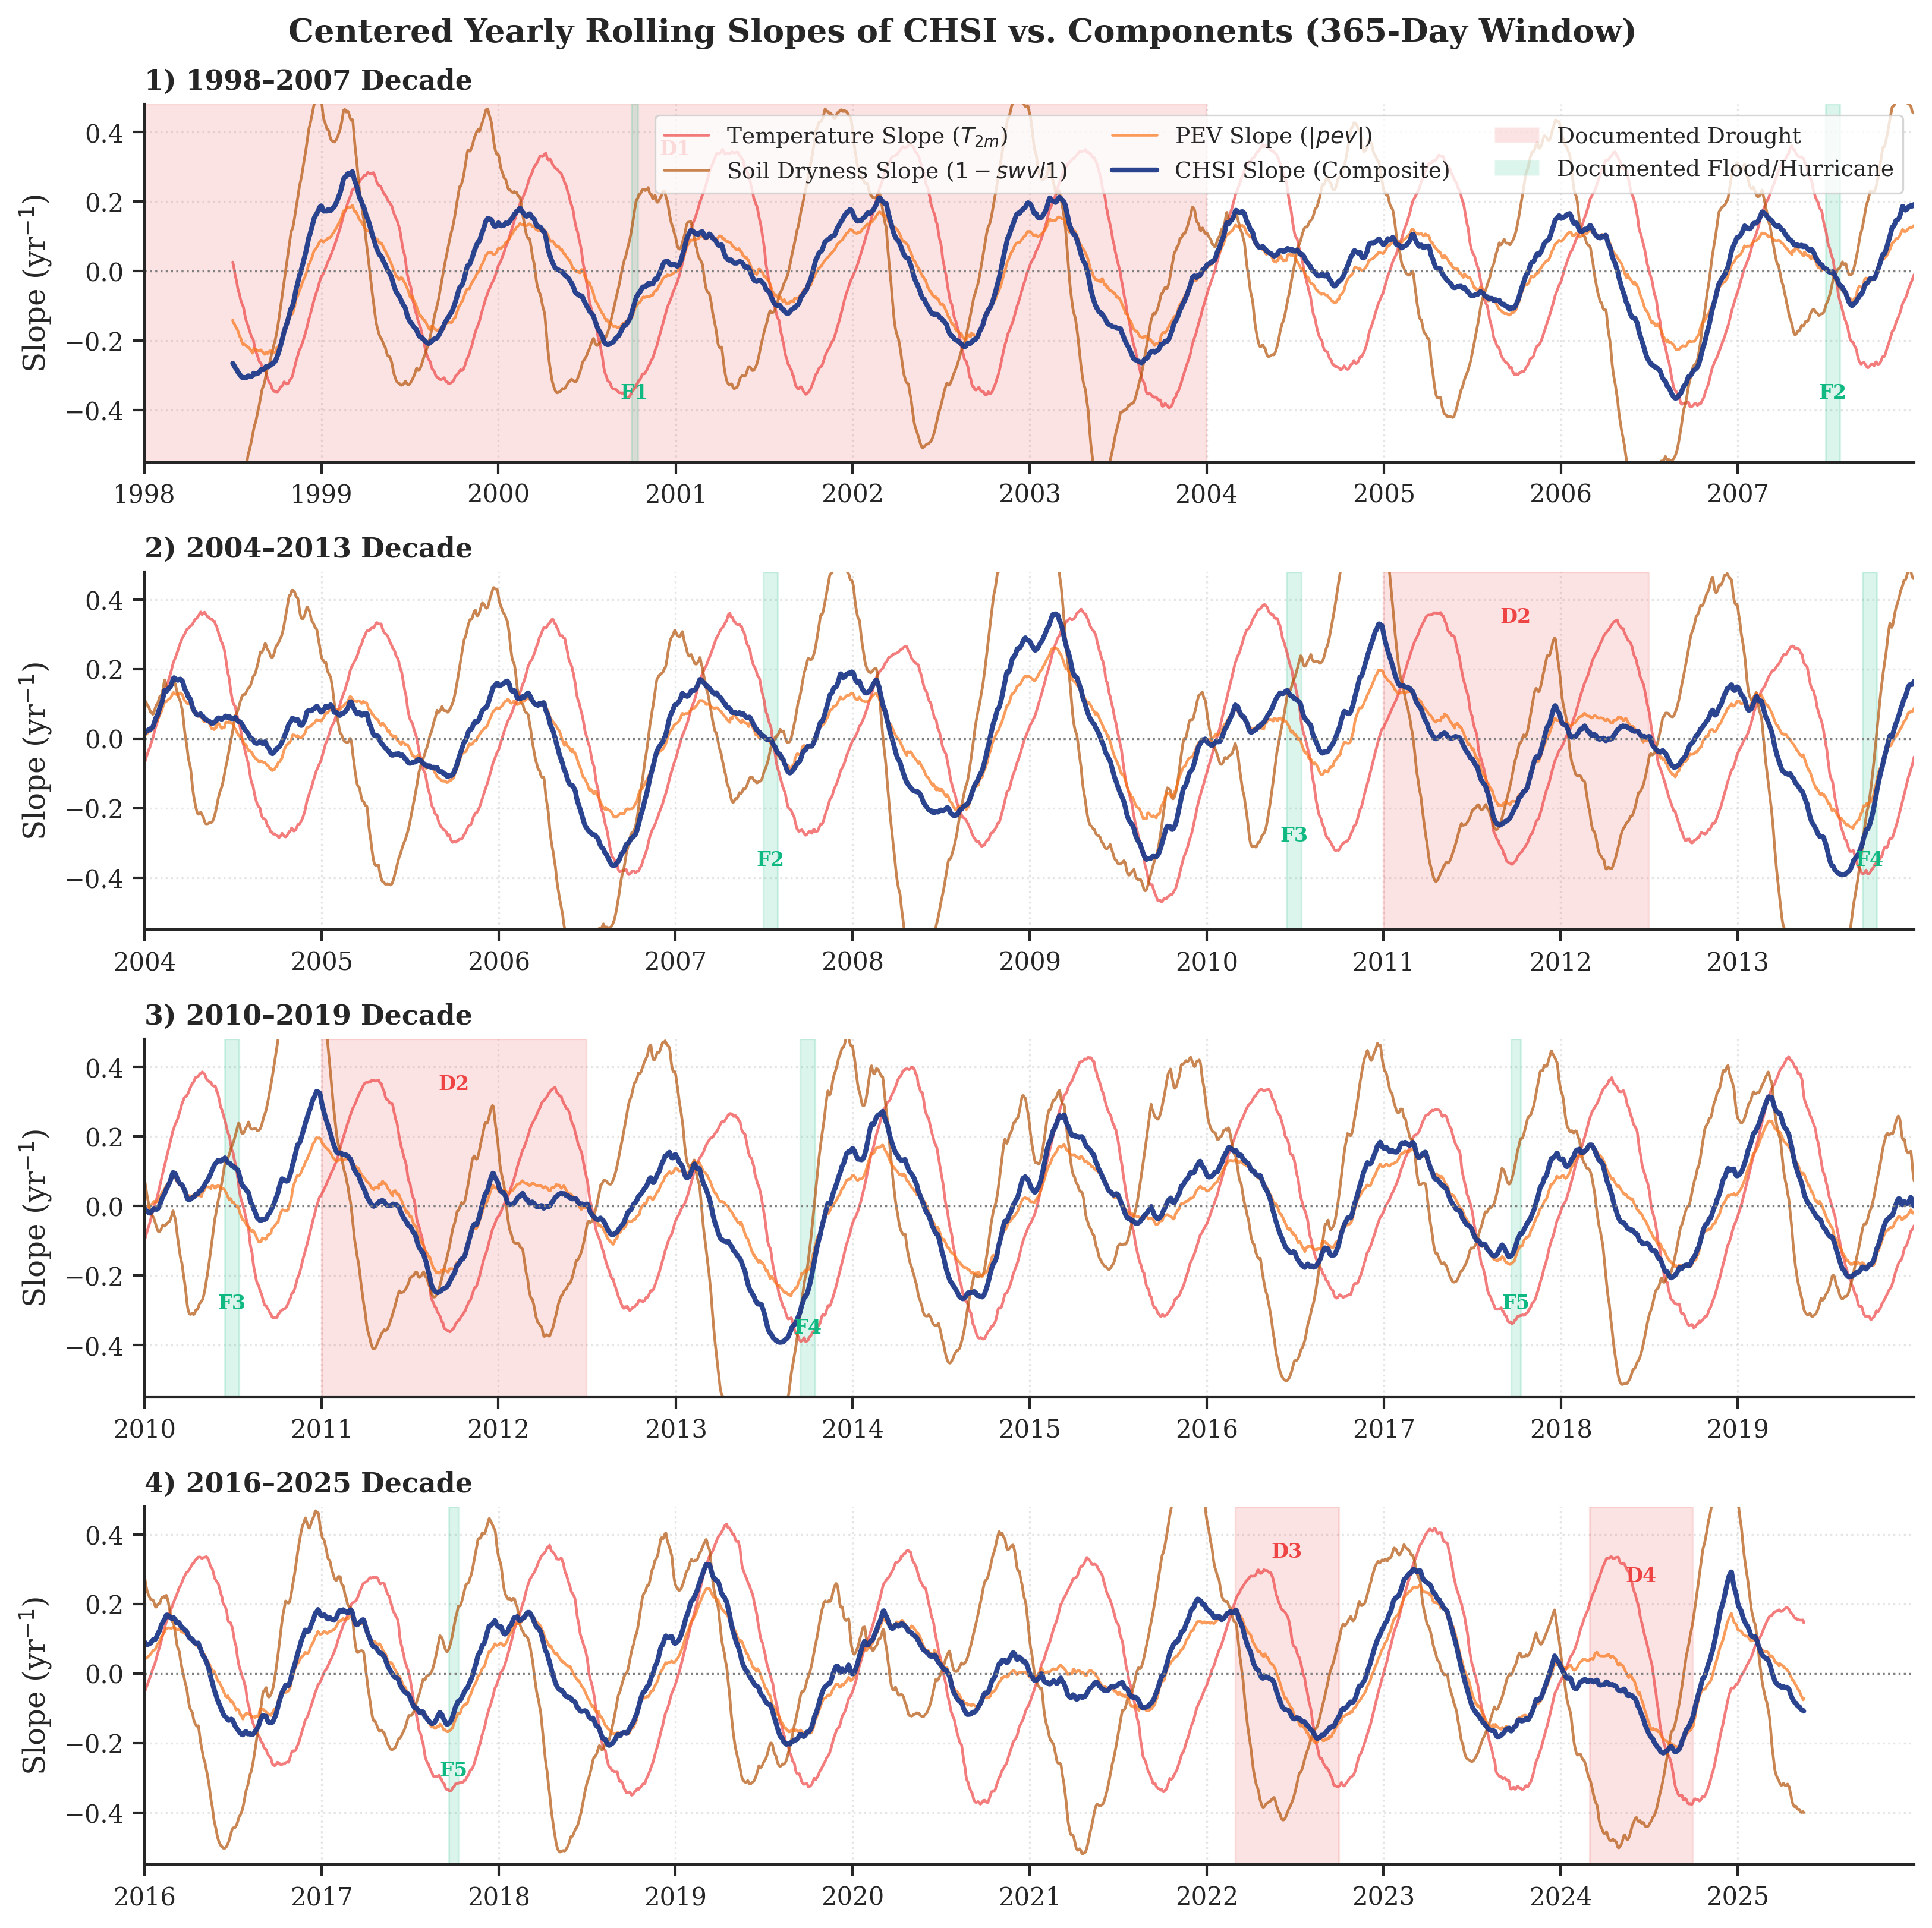
\includegraphics[width=\textwidth]{07_chsi_yearly_slopes_comparison.png}
    \caption{Pendientes de regresión anual centrada (ventana de 365~días) del CHSI y sus componentes normalizados, segmentadas en tres paneles cronológicos.}
    \label{fig:yearly_slopes}
\end{figure}

\subsection{CHSI reconstruido frente a estados de los componentes normalizados}
\label{subsec:components}

La Figura~\ref{fig:components} presenta el promedio móvil centrado de 30~días del CHSI normalizado junto con sus componentes individuales. Durante las sequías excepcionales de 2022 y 2024, el CHSI se mantiene consistentemente por encima de 0.60, impulsado por una sequedad edáfica ($1 - swvl1$) superior a 0.70 y una evaporación potencial elevada. Durante eventos de inundación, el índice desciende por debajo de 0.35 conforme la sequedad edáfica se aproxima a 0.15 por saturación.

\begin{figure}[H]
    \centering
    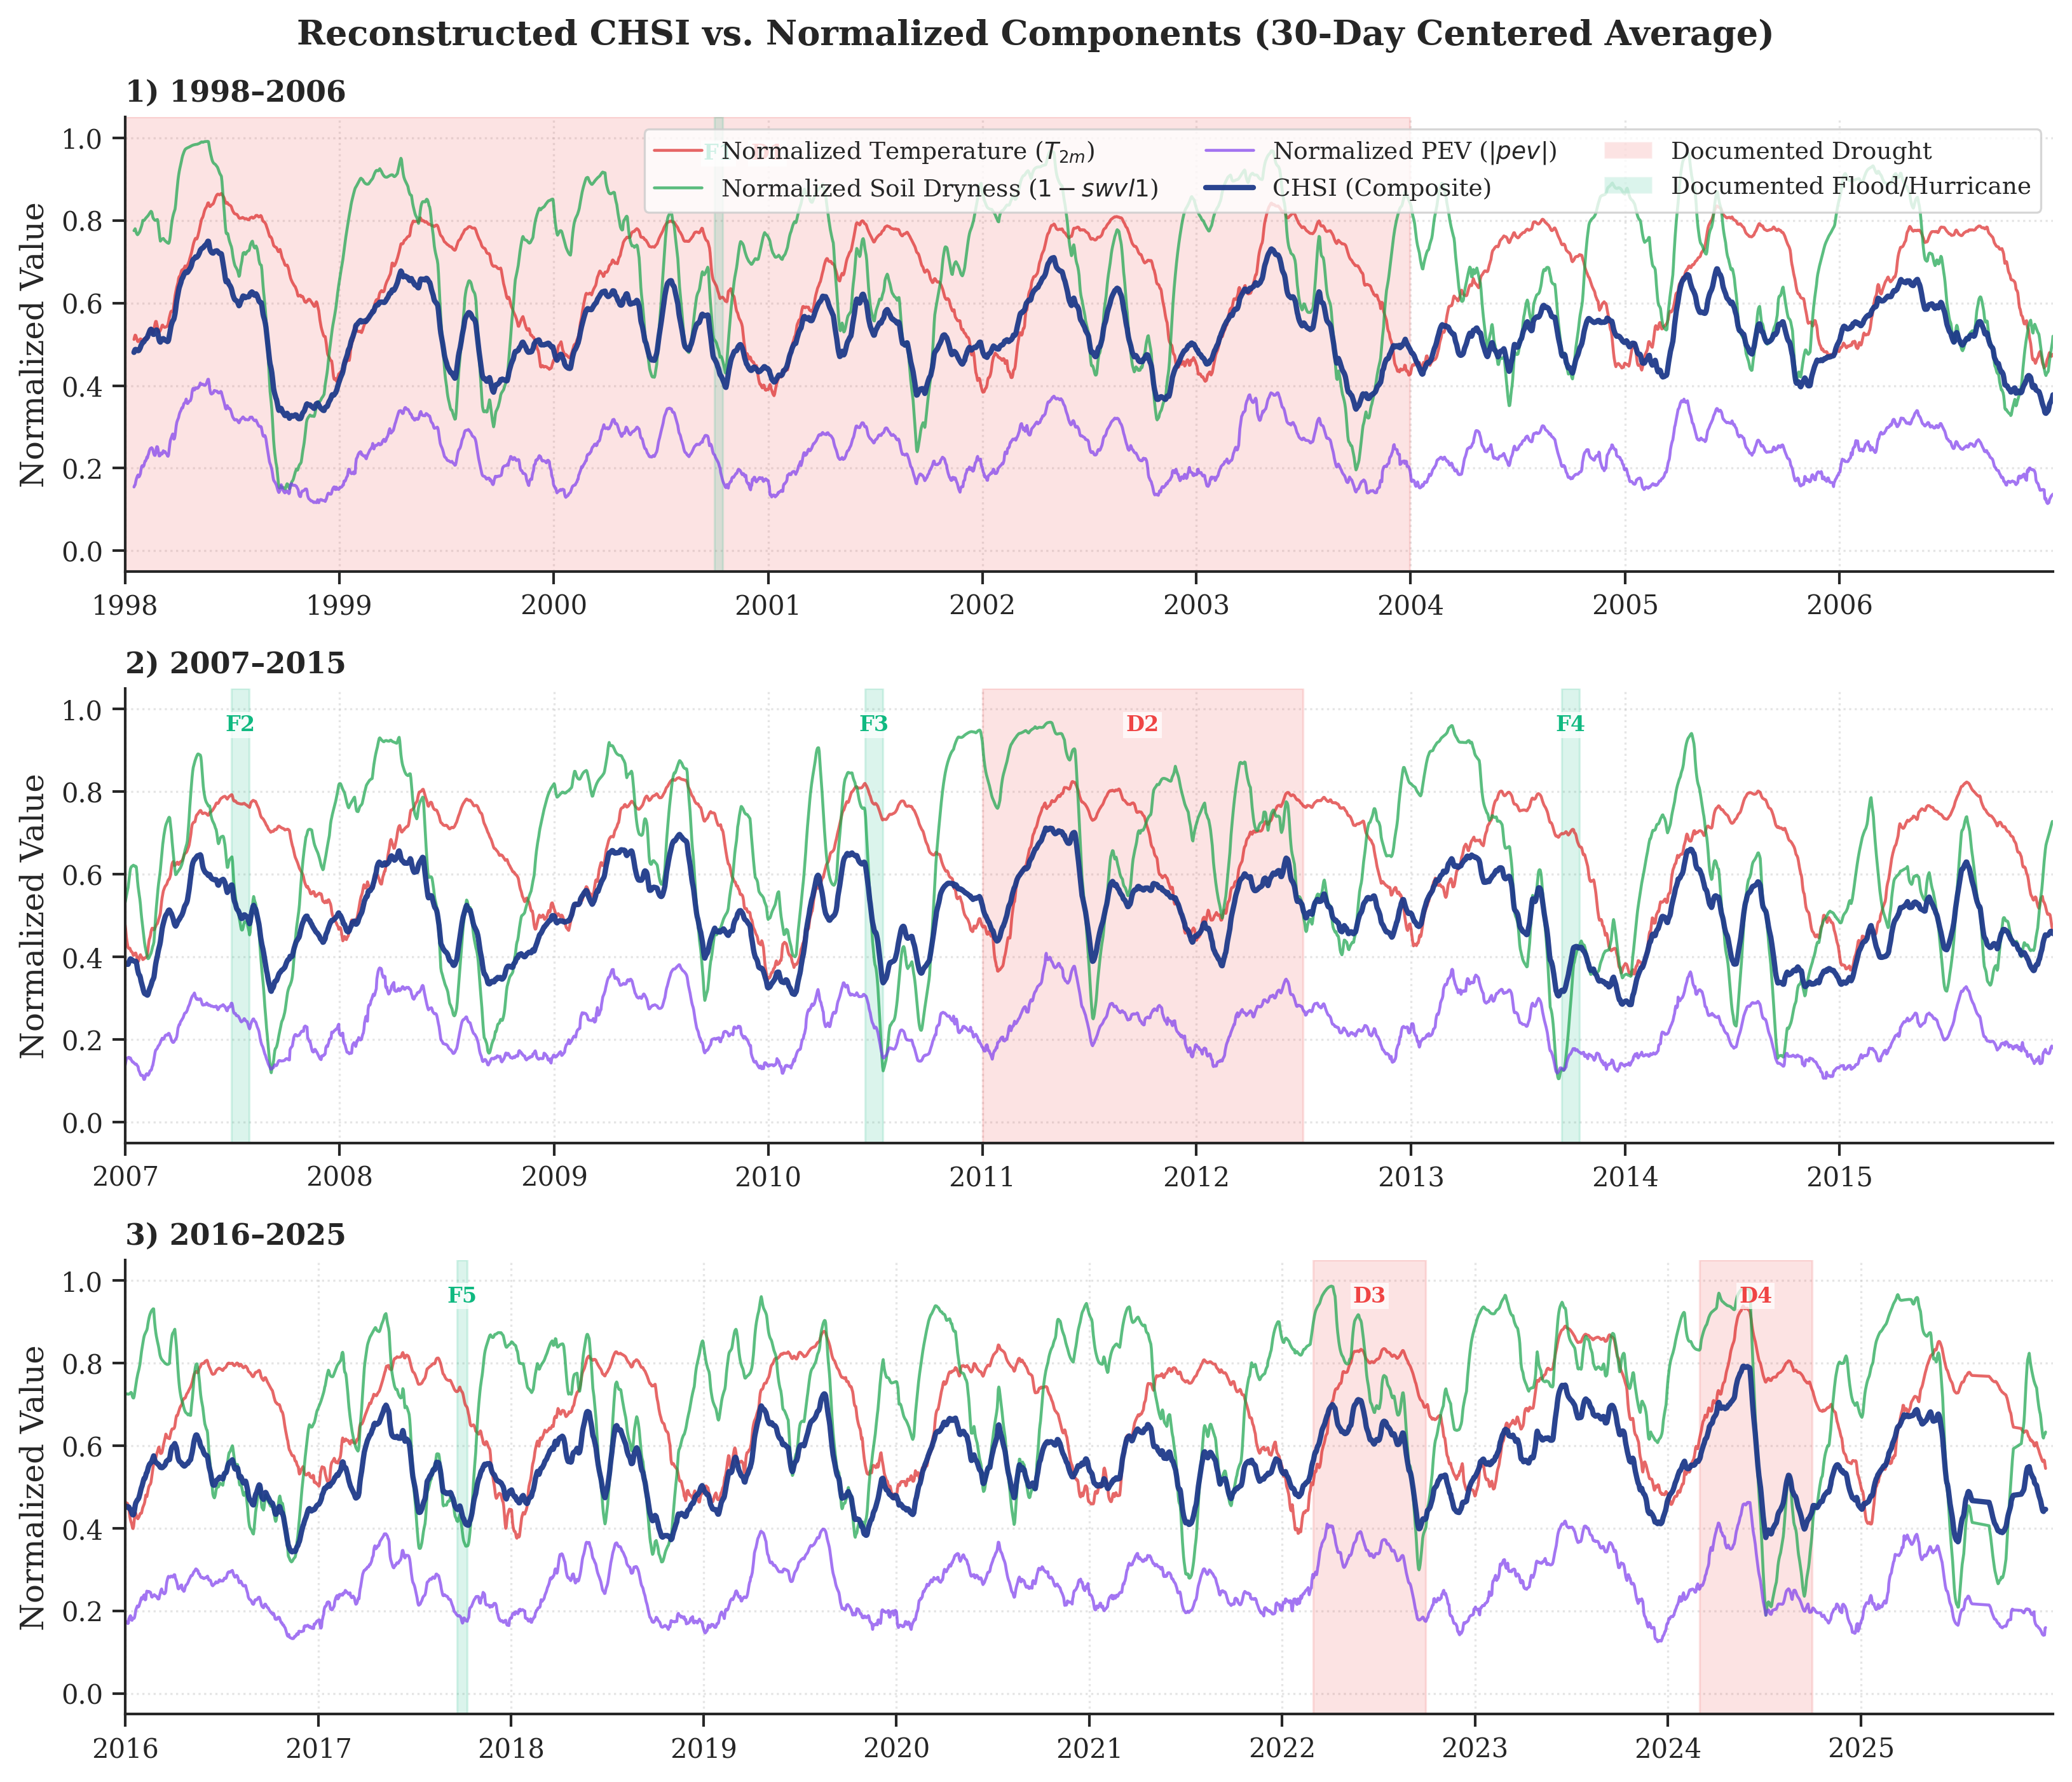
\includegraphics[width=\textwidth]{08_chsi_normalized_components_comparison.png}
    \caption{CHSI reconstruido frente a sus componentes normalizados (promedio centrado de 30~días), segmentado en tres paneles cronológicos. Los eventos de sequía (D1--D4) e inundación (F1--F5) se indican con bandas sombreadas.}
    \label{fig:components}
\end{figure}

\subsection{Régimen hidrológico y análisis de tendencias pre- y post-evento}
\label{subsec:regimen}

Se analizaron las tendencias lineales del CHSI bajo distintos regímenes hidrológicos: durante sequías documentadas (D1--D4) frente a periodos de línea base (fuera de sequías). Adicionalmente, se realizó un Análisis de Época Superpuesta (\emph{Superposed Epoch Analysis}, SEA) para examinar el comportamiento de la tasa de cambio del estrés antes y después del inicio de los eventos húmedos extremos (Figuras~\ref{fig:sea} y~\ref{fig:overlay}).

\begin{table}[H]
\centering
\caption{Estadísticos de regresión del CHSI por régimen ambiental y ventanas de anticipación/retraso respecto a eventos extremos}
\label{tab:regimen}
\small
\begin{tabular}{@{}lcccl@{}}
\toprule
Régimen / Ventana & Pendiente (año$^{-1}$) & $R^2$ & $p$ & Interpretación física \\
\midrule
Durante sequía              & $+0.005713$ & 0.0137 & $<0.0001$ & Aceleración del desecamiento \\
Fuera de sequía             & $+0.002712$ & 0.0167 & $<0.0001$ & Línea base de desecamiento gradual \\
1~año pre-inundación        & $+0.064908$ & 0.0248 & $<0.0001$ & Acumulación de estrés pre-evento \\
1~año post-inundación       & $+0.118477$ & 0.0801 & $<0.0001$ & Velocidad de recuperación post-evento \\
2~años pre-inundación       & $+0.023604$ & 0.0139 & $<0.0001$ & Acumulación de estrés pre-evento \\
2~años post-inundación      & $+0.042680$ & 0.0433 & $<0.0001$ & Velocidad de recuperación post-evento \\
5~años pre-inundación       & $+0.004290$ & 0.0026 & $<0.0001$ & Acumulación de estrés pre-evento \\
5~años post-inundación      & $+0.006620$ & 0.0067 & $<0.0001$ & Velocidad de recuperación post-evento \\
\bottomrule
\end{tabular}
\end{table}

Durante los periodos de sequía documentados, el estrés hídrico se acumula a una tasa de $+0.005713$~año$^{-1}$ ($p < 0.0001$), más del doble de la tasa observada fuera de sequías ($+0.002712$~año$^{-1}$). En los años previos a los ciclones tropicales, la cuenca registra pendientes positivas ($+0.064908$~año$^{-1}$ en la ventana de 1~año), lo que indica que las inundaciones en esta región tienden a ocurrir al final de ciclos secos severos, actuando como eventos de ruptura de sequía. Inmediatamente después del inicio de una inundación, el CHSI exhibe una tendencia positiva pronunciada ($+0.118477$~año$^{-1}$), que representa la \emph{velocidad de relajación y recuperación hidrológica} de la cuenca hacia su estado basal.

\begin{figure}[H]
    \centering
    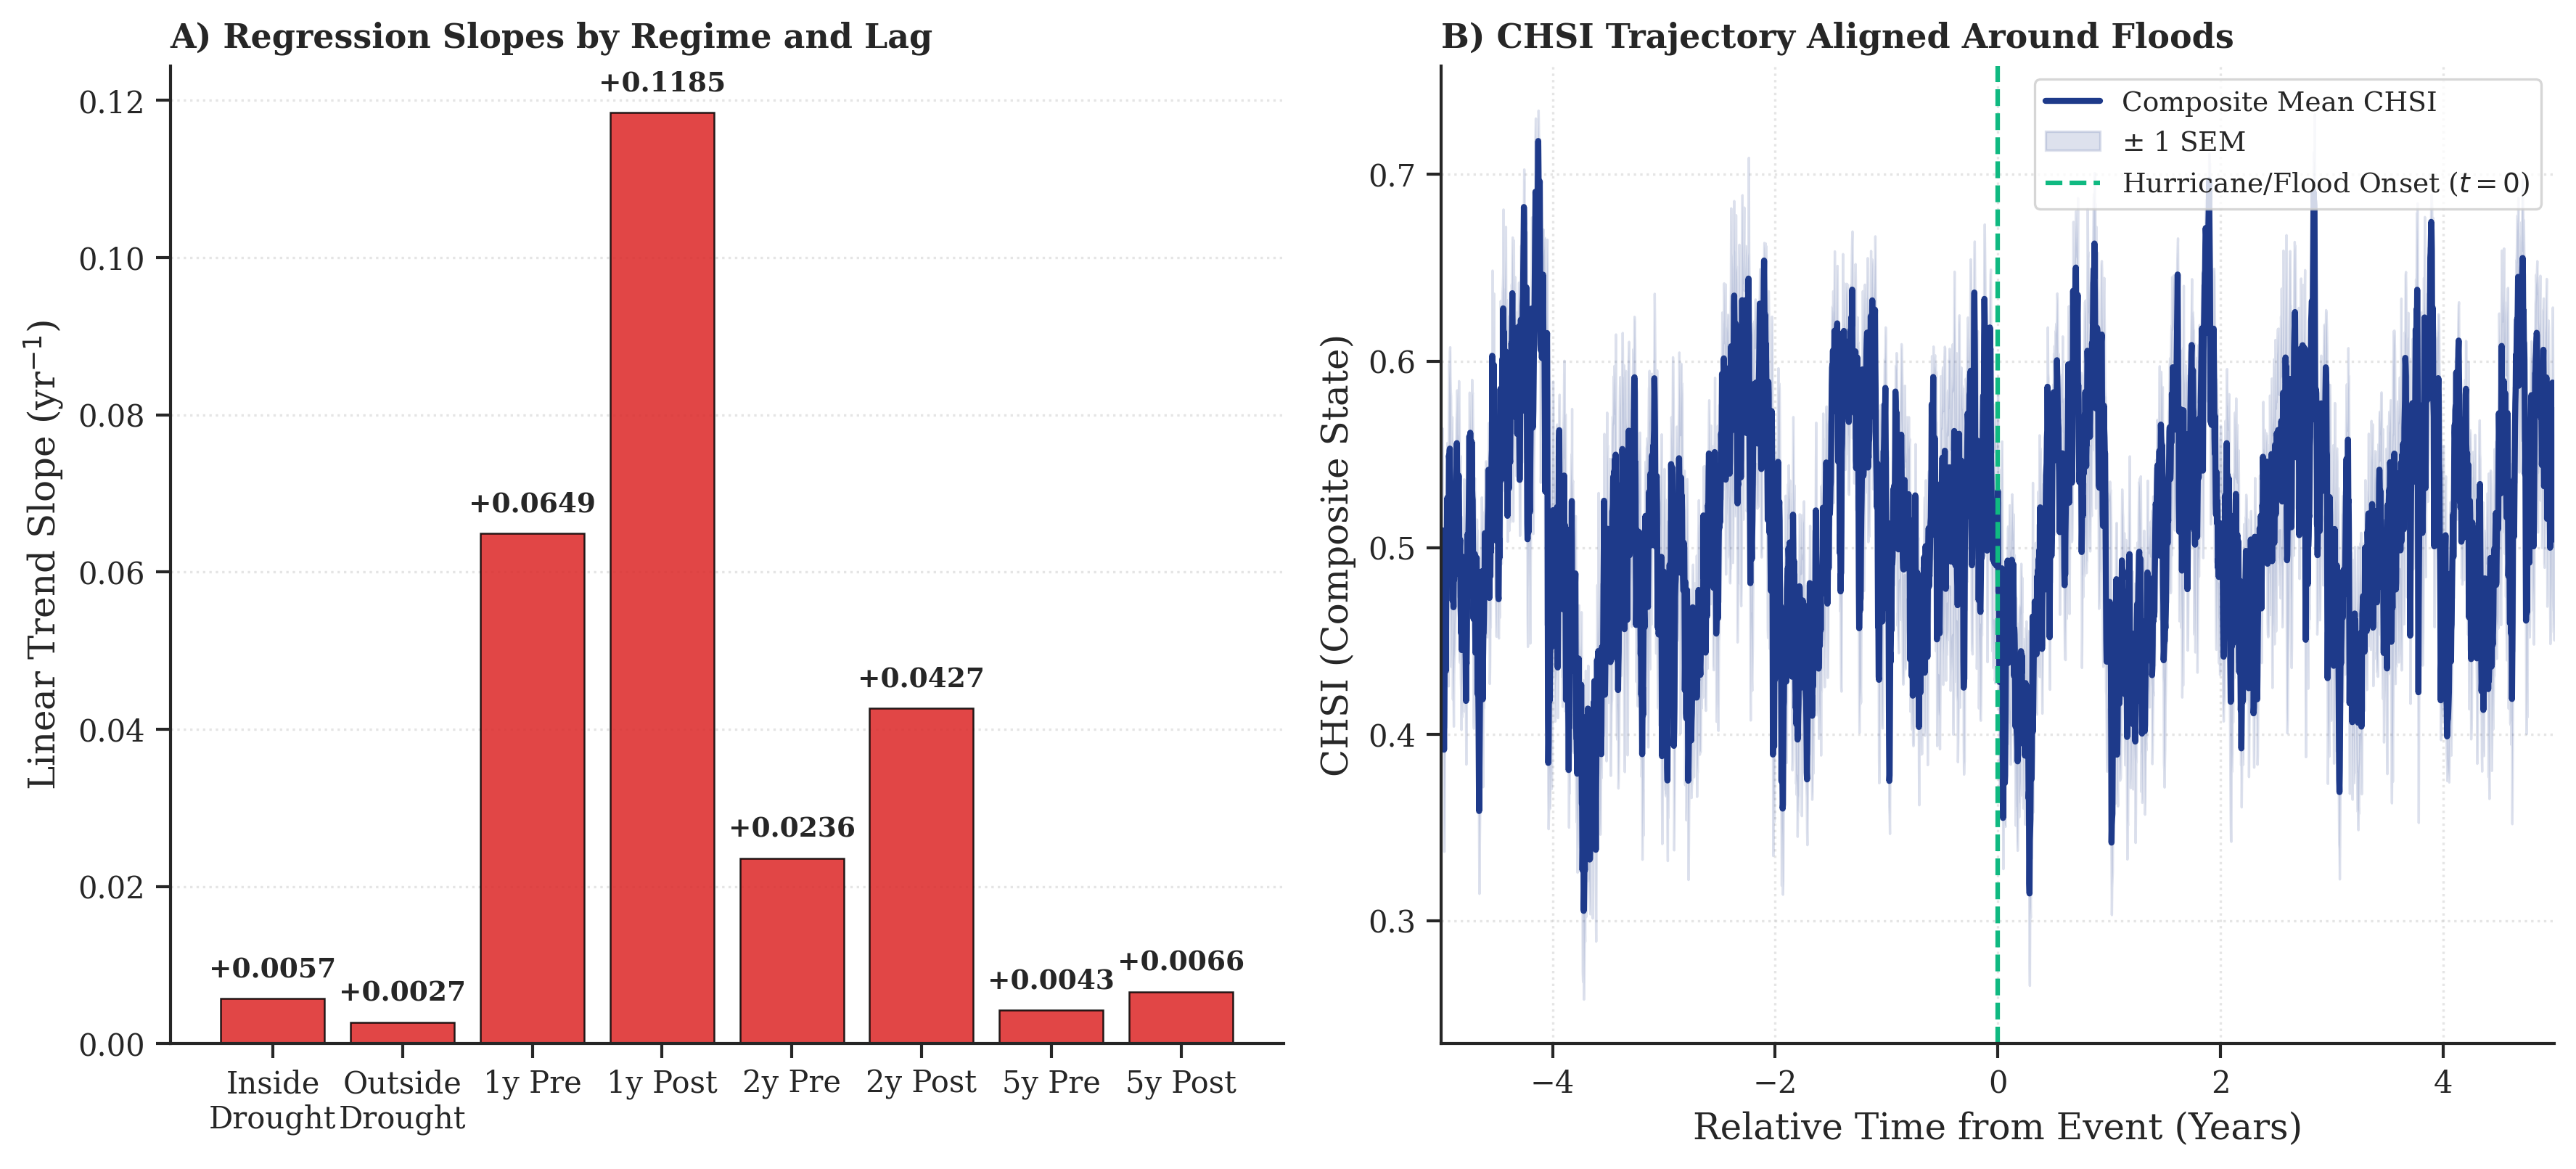
\includegraphics[width=\textwidth]{09_chsi_event_regime_sea_composite.png}
    \caption{Pendientes de regresión del CHSI por régimen hidrológico y análisis de época superpuesta (SEA) alineado al inicio de los eventos de inundación.}
    \label{fig:sea}
\end{figure}

\begin{figure}[H]
    \centering
    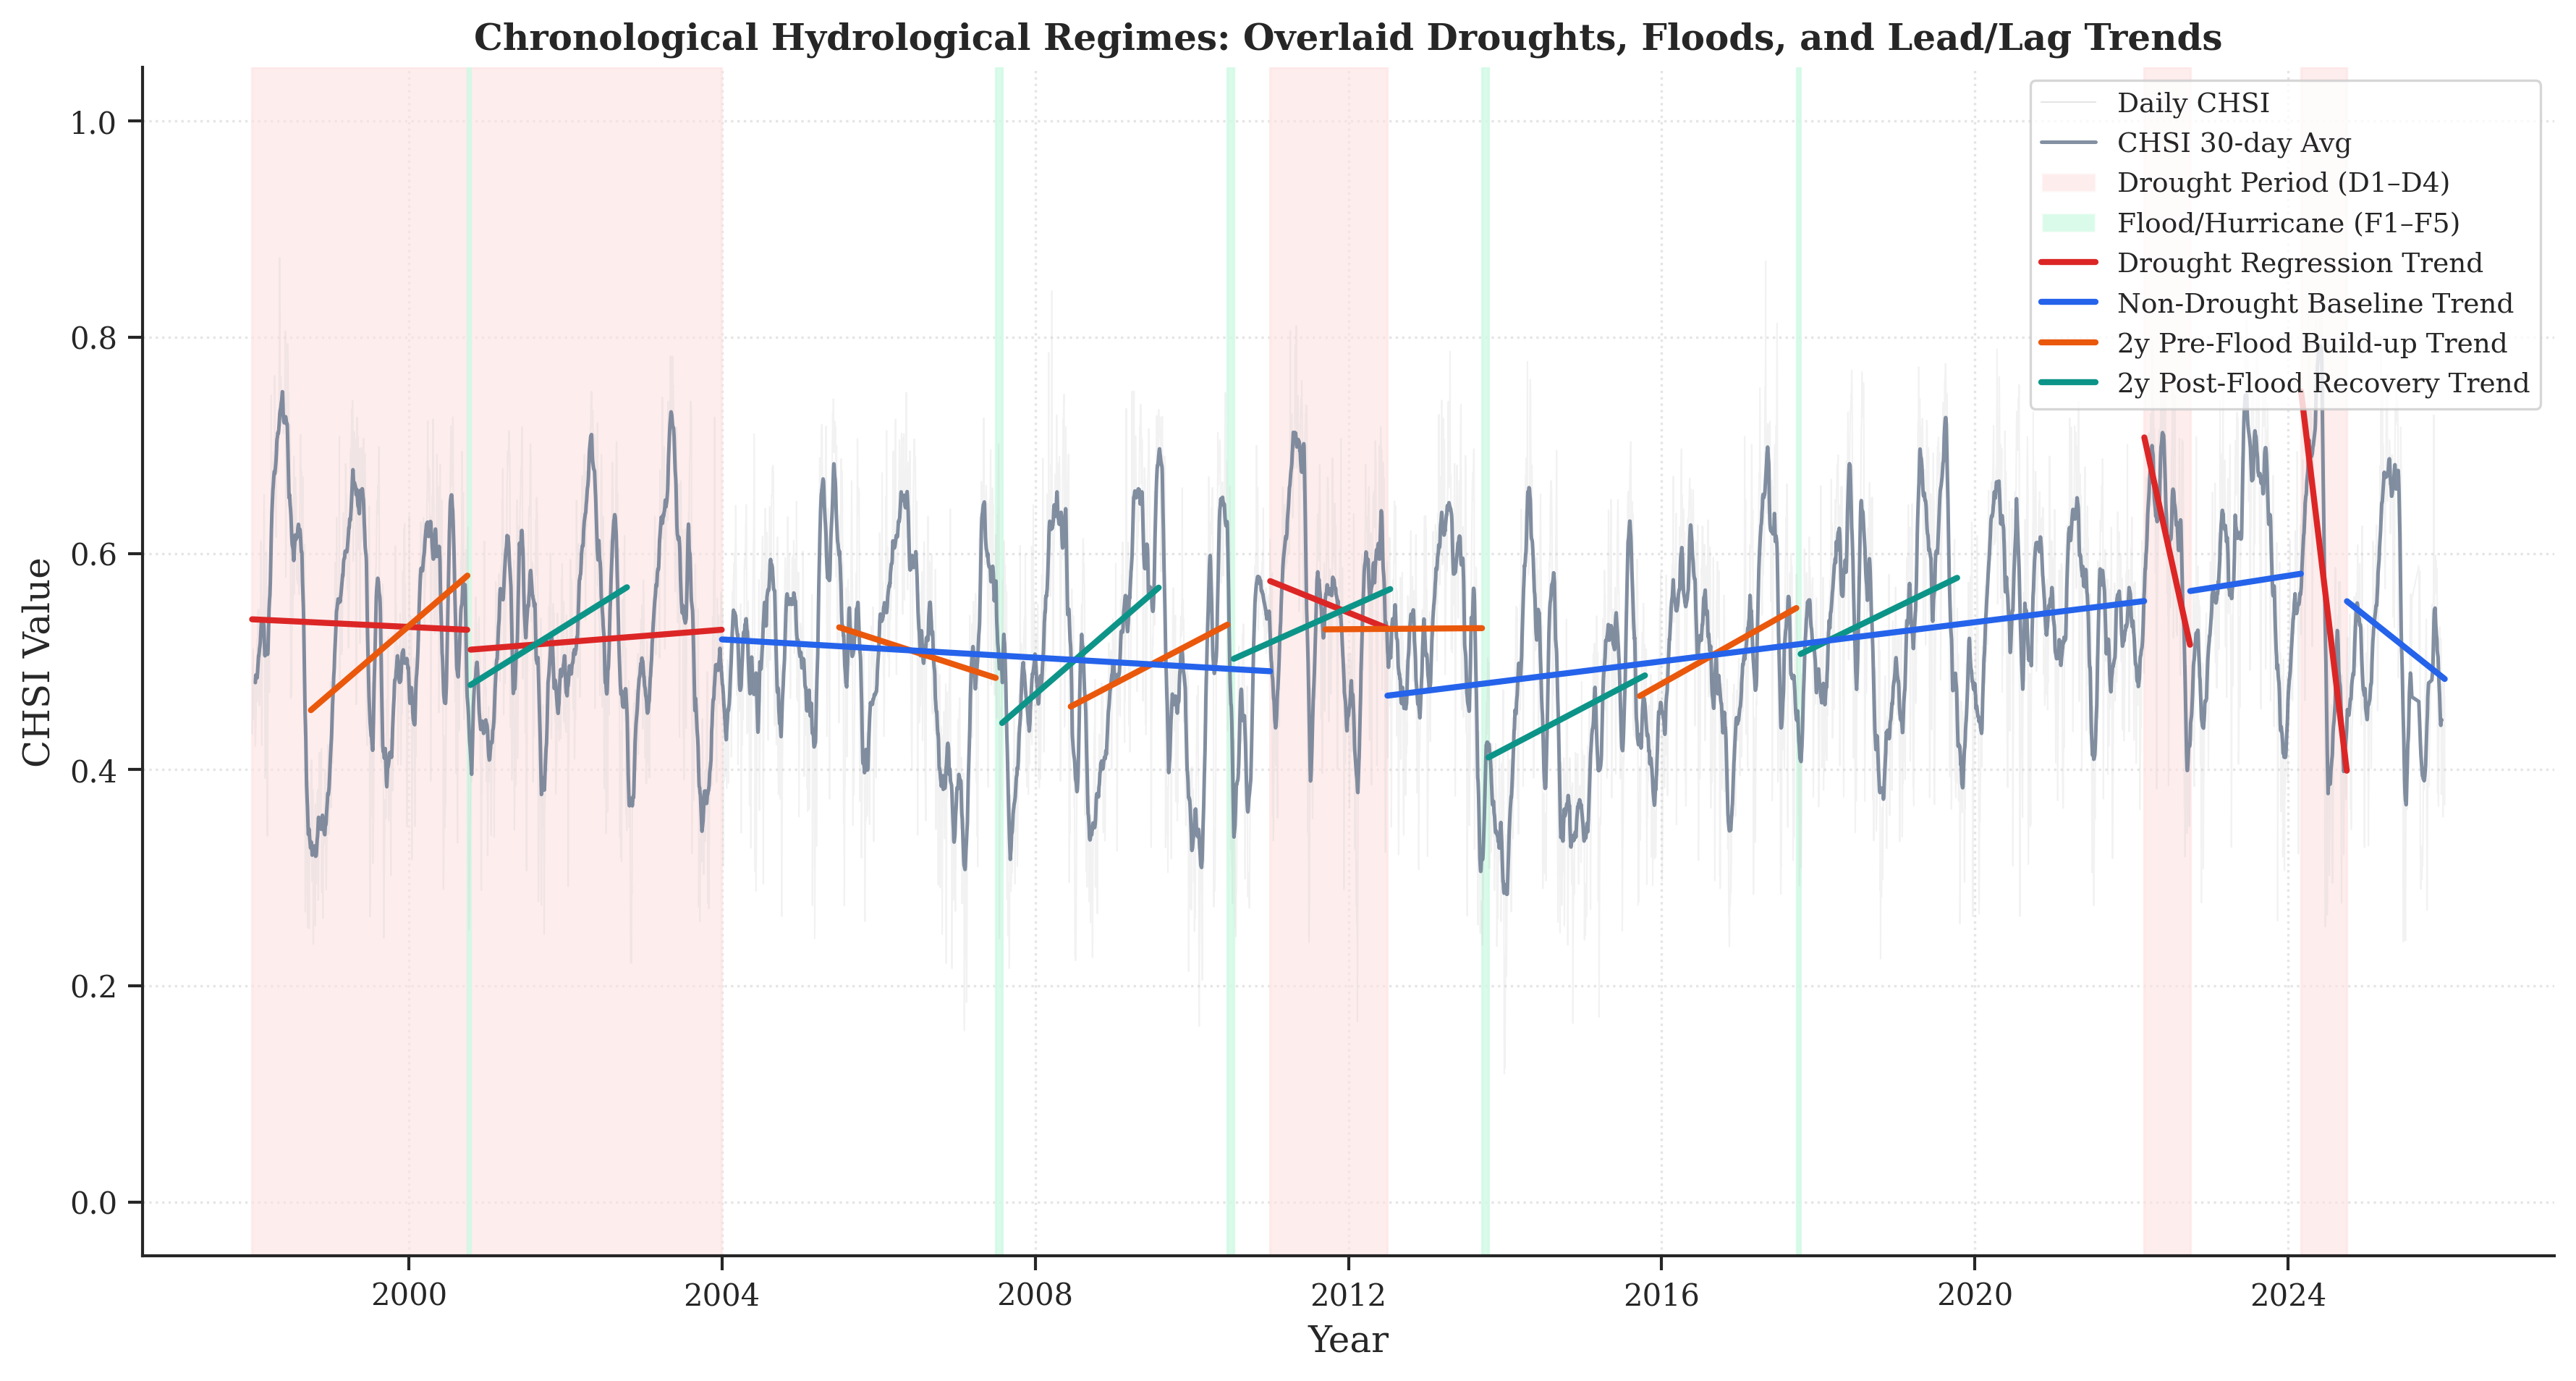
\includegraphics[width=\textwidth]{10_chsi_event_regime_chronological_overlay.png}
    \caption{Superposición cronológica de los segmentos de regresión del CHSI sobre la serie temporal completa (1998--2025). Segmentos rojos: periodos de sequía; segmentos azules: línea base; segmentos naranja/turquesa: ventanas pre- y post-inundación.}
    \label{fig:overlay}
\end{figure}

% ============================================================
\section{Discusión}
\label{sec:discusion}
% ============================================================

Los resultados obtenidos tienen implicaciones relevantes tanto para la gestión de recursos hídricos en el sur de Tamaulipas como para la metodología de inferencia de parámetros hidrológicos no observables.

\subsection{Calentamiento regional y aceleración de la demanda evaporativa}

La tendencia de calentamiento significativa de $+0.0387\,^\circ$C/año en la cuenca del Tamesí, acoplada con el incremento de la magnitud de la evaporación potencial, indica que la demanda evaporativa atmosférica se está acelerando. Aun si la precipitación permaneciera relativamente estable, este calentamiento incrementa la tasa de extracción de humedad del suelo, favoreciendo el inicio acelerado de sequías agrícolas y ecológicas, fenómeno descrito en la literatura como sequía repentina (\emph{flash drought}) \parencite{otkin2018flash}. El análisis de tendencias por ventana móvil (Figuras~\ref{fig:seasonal_slopes} y~\ref{fig:yearly_slopes}) confirma este comportamiento: la pendiente estacional de temperatura muestra pulsos de calentamiento de corto plazo, mientras que la pendiente anual máxima del CHSI ($+0.35861$~año$^{-1}$, centrada en febrero de~2009) revela una transición multianual sostenida hacia condiciones de desecamiento severo, impulsada por la depleción de humedad edáfica ($+0.54017$~año$^{-1}$) y la demanda evaporativa ($+0.25990$~año$^{-1}$).

\subsection{El CHSI como herramienta diagnóstica}

La validación mediante puntuaciones~$Z$ demuestra que el CHSI constituye un indicador sensible del estado hidrológico a escala de cuenca. Las sequías severas de~2022 ($Z = +0.832$) y~2024 ($Z = +0.494$) son capturadas con claridad, al igual que los eventos de inundación, cuyos valores~$Z$ negativos pronunciados (por ejemplo, $-1.079$ durante el huracán Ingrid) reflejan la saturación rápida del suelo y el enfriamiento superficial asociado. La comparación de las pendientes anuales centradas (Figura~\ref{fig:yearly_slopes}) y los estados de las variables componentes (Figura~\ref{fig:components}) sugieren que la cuenca del Tamesí se encuentra en su ciclo de desecamiento multianual más sostenido desde el inicio del registro, con pendientes anuales elevadas persistentes durante el periodo 2018--2024. Esta respuesta dinámica diferenciada y la sensibilidad para capturar tanto la firma de sequías prolongadas como el exceso hídrico transitorio es consistente con los hallazgos de \textcite{rostami2025simulating}, quienes demuestran la viabilidad de utilizar modelado basado en datos y análisis de series de tiempo para simular inundaciones compuestas y el impacto de ciclones tropicales en zonas costeras vulnerables, sirviendo como proxy del estado hidrológico integrado.

\subsection{Contraste con metodologías y métricas alternativas}

El desarrollo del CHSI ofrece ventajas distintivas al compararse con metodologías tradicionales e índices convencionales de sequía y estrés hídrico. Los índices meteorológicos como el SPI \parencite{mckee1993relationship} o el SPEI \parencite{vicente2010multiscalar} se calculan de manera puramente estadística a partir de datos de precipitación y temperatura acumulados en ventanas temporales fijas. Aunque son útiles para caracterizar anomalías a escala regional, ignoran por completo el estado del suelo y el acoplamiento termodinámico con la vegetación, lo que limita su capacidad para representar el estrés fisiológico real en la cuenca. Al integrar directamente el contenido de agua edáfica superficial ($swvl1$), el CHSI captura no solo la falta de lluvia, sino la respuesta del suelo y su interacción con la atmósfera.

Por otra parte, el Monitor de Sequía de México (MSM) de la CONAGUA utiliza el modelo conceptual \emph{Leaky Bucket} de una sola capa \parencite{lobato2016monitor}. Si bien este modelo representa un avance al estimar la humedad del suelo, carece de acoplamiento con las variaciones de temperatura y demanda evaporativa a escalas temporales de alta resolución (sub-diarias u horarias). El CHSI, derivado de ERA5-Land, aprovecha la asimilación de datos físicos continuos y modela el triángulo de estrés (energía, agua en el suelo y demanda atmosférica) de forma acoplada.

Frente a metodologías basadas exclusivamente en sensores remotos ópticos, como el Índice de Estrés Hídrico de la Vegetación (VSWI) o el Índice Multibanda Normalizado de Sequía (NMDI) de \textcite{ghafari2024spatial}, que dependen de la reflectancia en las bandas del infrarrojo cercano y de onda corta, el CHSI basado en reanálisis presenta una cobertura temporal continua y libre de la interferencia por nubosidad, una limitación crítica en las cuencas costeras del Golfo de México durante la temporada de ciclones. Además, a diferencia de los índices puramente empíricos, los estimadores no lineales desarrollados (GBR y RF) permiten emular estas dinámicas sin requerir la presencia de variables físicas primarias en tiempo real, validando al CHSI como un emulador dinámico viable para la transferencia espacial.

\subsection{Selección del modelo y ganancia del aprendizaje secuencial}

La comparación entre el RF y el GBR demuestra que el \emph{boosting} ofrece una ventaja determinante en la modelación del estrés hídrico. Si bien el enfoque de \emph{bagging} del RF proporciona una línea base robusta, el GBR reduce el error de predicción (RMSE) en un 37.9\,\%. El mecanismo de \emph{boosting} construye árboles secuenciales que se enfocan en reducir los residuos de iteraciones previas, lo que le permite capturar con mayor precisión las condiciones de frontera, tales como las transiciones rápidas hacia sequías repentinas o la saturación máxima durante el paso de ciclones tropicales, que los modelos de \emph{bagging} tienden a suavizar.

\subsection{Interpretabilidad física mediante SHAP}

Mediante la extracción de valores SHAP se supera el sesgo de la importancia estándar de Gini, que sobre-representa las variables continuas. El análisis SHAP revela un umbral no lineal en el acoplamiento suelo-atmósfera: cuando la humedad edáfica ($swvl1$) desciende por debajo de $0.22$~m$^3$/m$^3$, la contribución SHAP del índice térmico-hídrico ($T_{2m}/\theta_{\text{swvl1}}$) se incrementa de forma exponencial. Este comportamiento modela la transición desde un régimen de evapotranspiración limitado por energía hacia un régimen limitado por agua, proporcionando una explicación física de las retroalimentaciones suelo-atmósfera consistente con el marco teórico de \textcite{seneviratne2010investigating}.

\subsection{Dinámica de régimen hidrológico}

El análisis de regímenes (Tabla~\ref{tab:regimen}) revela que durante sequías documentadas el estrés se acumula al doble de la tasa observada en periodos normales. La pendiente positiva pre-inundación ($+0.064908$~año$^{-1}$ en la ventana de 1~año) indica que los ciclones tropicales en esta cuenca tienden a ocurrir tras ciclos secos prolongados, funcionando como eventos de ruptura de sequía. La elevada pendiente post-inundación ($+0.118477$~año$^{-1}$) cuantifica la velocidad de relajación hidrológica de la cuenca: la inundación deposita un exceso de humedad que se disipa rápidamente bajo las condiciones de alta demanda evaporativa propias de la región, retornando al estado basal climatológico en uno a dos años.

\subsection{Integración con la línea de investigación doctoral}

Un cuello de botella recurrente en la teledetección de recursos hídricos radica en que las observaciones satelitales (reflectancia óptica, retrodispersión de radar) son indirectas y están limitadas por la cobertura nubosa y los periodos de revisita. Los datos de reanálisis como ERA5-Land ofrecen registros continuos y de largo plazo, pero con resolución espacial gruesa (${\sim}9$~km). La metodología del CHSI funciona como una \emph{línea base de reducción de escala e inferencia}. El elevado desempeño del GBR ($R^2 > 0.99$) demuestra que el mapeo estadístico de las interacciones suelo-atmósfera es altamente aprendible. En la siguiente fase de esta línea de investigación, el modelo se adaptará para integrar entradas de teledetección satelital de alta resolución (NDVI de Sentinel-2, índice de humedad de Sentinel-1, evapotranspiración real de MODIS) con el objetivo de reducir la escala del CHSI desde 9~km hasta 10--100~m, habilitando el monitoreo de estrés hídrico a escala de parcela agrícola. Este enfoque de interpolación y downscaling espacial de la humedad superficial mediante el acoplamiento de sensores de microondas y ópticos con aprendizaje automático es consistente con estudios recientes de reducción de escala para productos de radiómetro satelital global como SMAP \parencite{ghafari2024spatial}.

% ============================================================
\section{Conclusiones}
\label{sec:conclusiones}
% ============================================================

En este estudio se derivó y validó el Índice Compuesto de Estrés Hídrico (CHSI) para la cuenca del río Guayalejo-Tamesí a partir de 28~años de datos horarios ERA5-Land y aprendizaje automático comparativo. El Regresor de Gradient Boosting (GBR) demostró ser superior al modelo de Bosque Aleatorio, explicando el 99.58\,\% de la varianza de la variable de respuesta y reduciendo el RMSE a 0.0072. El análisis de tendencias confirmó un calentamiento local significativo y un incremento de la demanda evaporativa potencial en el noreste de México. La validación frente a nueve eventos extremos documentados demostró la consistencia física y la capacidad diagnóstica del índice, con una concordancia direccional del 100\,\%. El análisis de régimen hidrológico reveló que la tasa de acumulación de estrés durante sequías duplica la observada en periodos normales, y que los ciclones tropicales actúan como eventos de ruptura tras ciclos de desecamiento prolongado.

Estos hallazgos establecen una línea base de reanálisis que valida la viabilidad de emplear aprendizaje automático para inferir parámetros hídricos complejos y no observables a partir de variables ambientales acopladas, sentando las bases para la reducción de escala con teledetección satelital de alta resolución.

% ============================================================
% Referencias
% ============================================================
\newpage
\printbibliography[title={Referencias}]

\end{document}
